\documentclass[11pt,twoside,openright]{report}

\usepackage[czech,english]{babel}
\usepackage{lmodern}
\usepackage[T1]{fontenc}
\usepackage{kpfonts}
\usepackage[utf8]{inputenc}
\usepackage[a4paper,width=150mm,top=25mm,bottom=25mm]{geometry}
\usepackage{graphicx}
\graphicspath{ {images/} }

\usepackage{emptypage}
\usepackage{fancyhdr}
\pagestyle{fancy}
\fancyhead{}
\fancyhead[RO,LE]{\leftmark}
\fancyfoot{}
\fancyfoot[C]{\thepage}

\usepackage{epstopdf}

\usepackage[nottoc]{tocbibind}
\usepackage[authoryear,round]{natbib}

\usepackage{float}

\usepackage{datetime}
\usepackage[pdftex,final]{hyperref}

\usepackage{algorithm}
\usepackage{algpseudocode}
\usepackage{amsmath}
\usepackage{amsfonts}
\usepackage{amssymb}
\usepackage{mathtools}
\usepackage{interval}
\usepackage{enumitem}

\usepackage{caption}
\usepackage{booktabs}
\usepackage{color}
\usepackage{subcaption}

\usepackage{multirow}
\usepackage{pdfpages}

\usepackage{tikz}
\usepackage{bm}

\addto\extrasenglish{%
  \renewcommand{\chapterautorefname}{Chapter}%
  \renewcommand{\sectionautorefname}{Section}%
  \renewcommand{\subsectionautorefname}{Subsection}%
}

% Make autoref work for the algorithm environment.
\newcommand{\algorithmautorefname}{Algorithm}

%% Definitions %%

% ForEach loop
\algnewcommand\algorithmicforeach{\textbf{for each}}
\algdef{S}[FOR]{ForEach}[1]{\algorithmicforeach\ #1\ \algorithmicdo}

% Break
\newcommand{\Break}{\State \textbf{break} }

% Input
\algnewcommand\algorithmicinput{\textbf{Input:}}
\algnewcommand\Input{\item[\algorithmicinput]}

% Output
\algnewcommand\algorithmicoutput{\textbf{Output:}}
\algnewcommand\Output{\item[\algorithmicoutput]}

\newcommand{\R}{\mathbb{R}}  % Pretty set of real numbers.
\newcommand{\N}{\mathbb{N}}  % Pretty set of natural numbers.
\newcommand{\E}{\mathbb{E}}  % Pretty expectation.
\newcommand{\I}{\mathbb{I}}  % Pretty indicator function.
\DeclarePairedDelimiter{\ceil}{\lceil}{\rceil}  % The ceiling function.
\DeclarePairedDelimiter{\floor}{\lfloor}{\rfloor}  % The floor function.

\newcommand{\vect}[1]{\bm{\MakeLowercase{#1}}}  % Pretty vectors.
\newcommand{\mat}[1]{\mathbf{#1}}  % Pretty matrices.

\DeclareMathOperator*{\argmin}{argmin}  % Argmin
\DeclareMathOperator*{\argmax}{argmax}  % Argmax


\newcommand{\btheta}{\bm{\theta}}
\newcommand{\bx}{\bm{x}}
\newcommand{\by}{\bm{y}}
\newcommand{\bu}{\bm{u}}
\newcommand{\aux}{z}
\newcommand{\auxjoint}{\pi}
\newcommand{\A}{\mathcal{A}}

\newcommand{\trans}{f}
\newcommand{\obs}{g}
\newcommand{\sprior}{p}
\newcommand{\pprior}{\pi}
\newcommand{\prop}{q}
\newcommand{\dx}[1]{\mathrm{d}{#1}}


%% Title %%
\newcommand*{\myTitle}{\begingroup 
    \centering 
    \vspace*{\baselineskip} 
    
    
    {\large Master Thesis} \\
    \vspace*{\baselineskip}
    {\LARGE Bayesian Parameter Estimation of State-Space Models with Intractable Likelihood}    
    \vspace*{5\baselineskip} 
    
    {\Large Bc. Tom\'{a}\v{s} Kala\par} 
    \scshape
    Supervisor: Ing. Kamil Dedecius, PhD.
    
    \vspace*{1\baselineskip}
    \monthname \ \the\year
    
    \vfill
    
    
\includegraphics[width=0.4\textwidth]{lion}
    
    \vspace*{1\baselineskip}
    Department of Computer Science\\
    Faculty of Electrical Engineering\\
    Czech Technical University in Prague\\[\baselineskip]
    
    \endgroup\cleardoublepage}


%% Document %%
\begin{document}
\selectlanguage{english}

% Title page
%\input{tex/titlepage}
\begin{titlepage}
\myTitle
\end{titlepage}

%\cleardoublepage
%\pagenumbering{roman}

% Assignment
\shorthandoff{-}  % Czech babel makes trouble here.
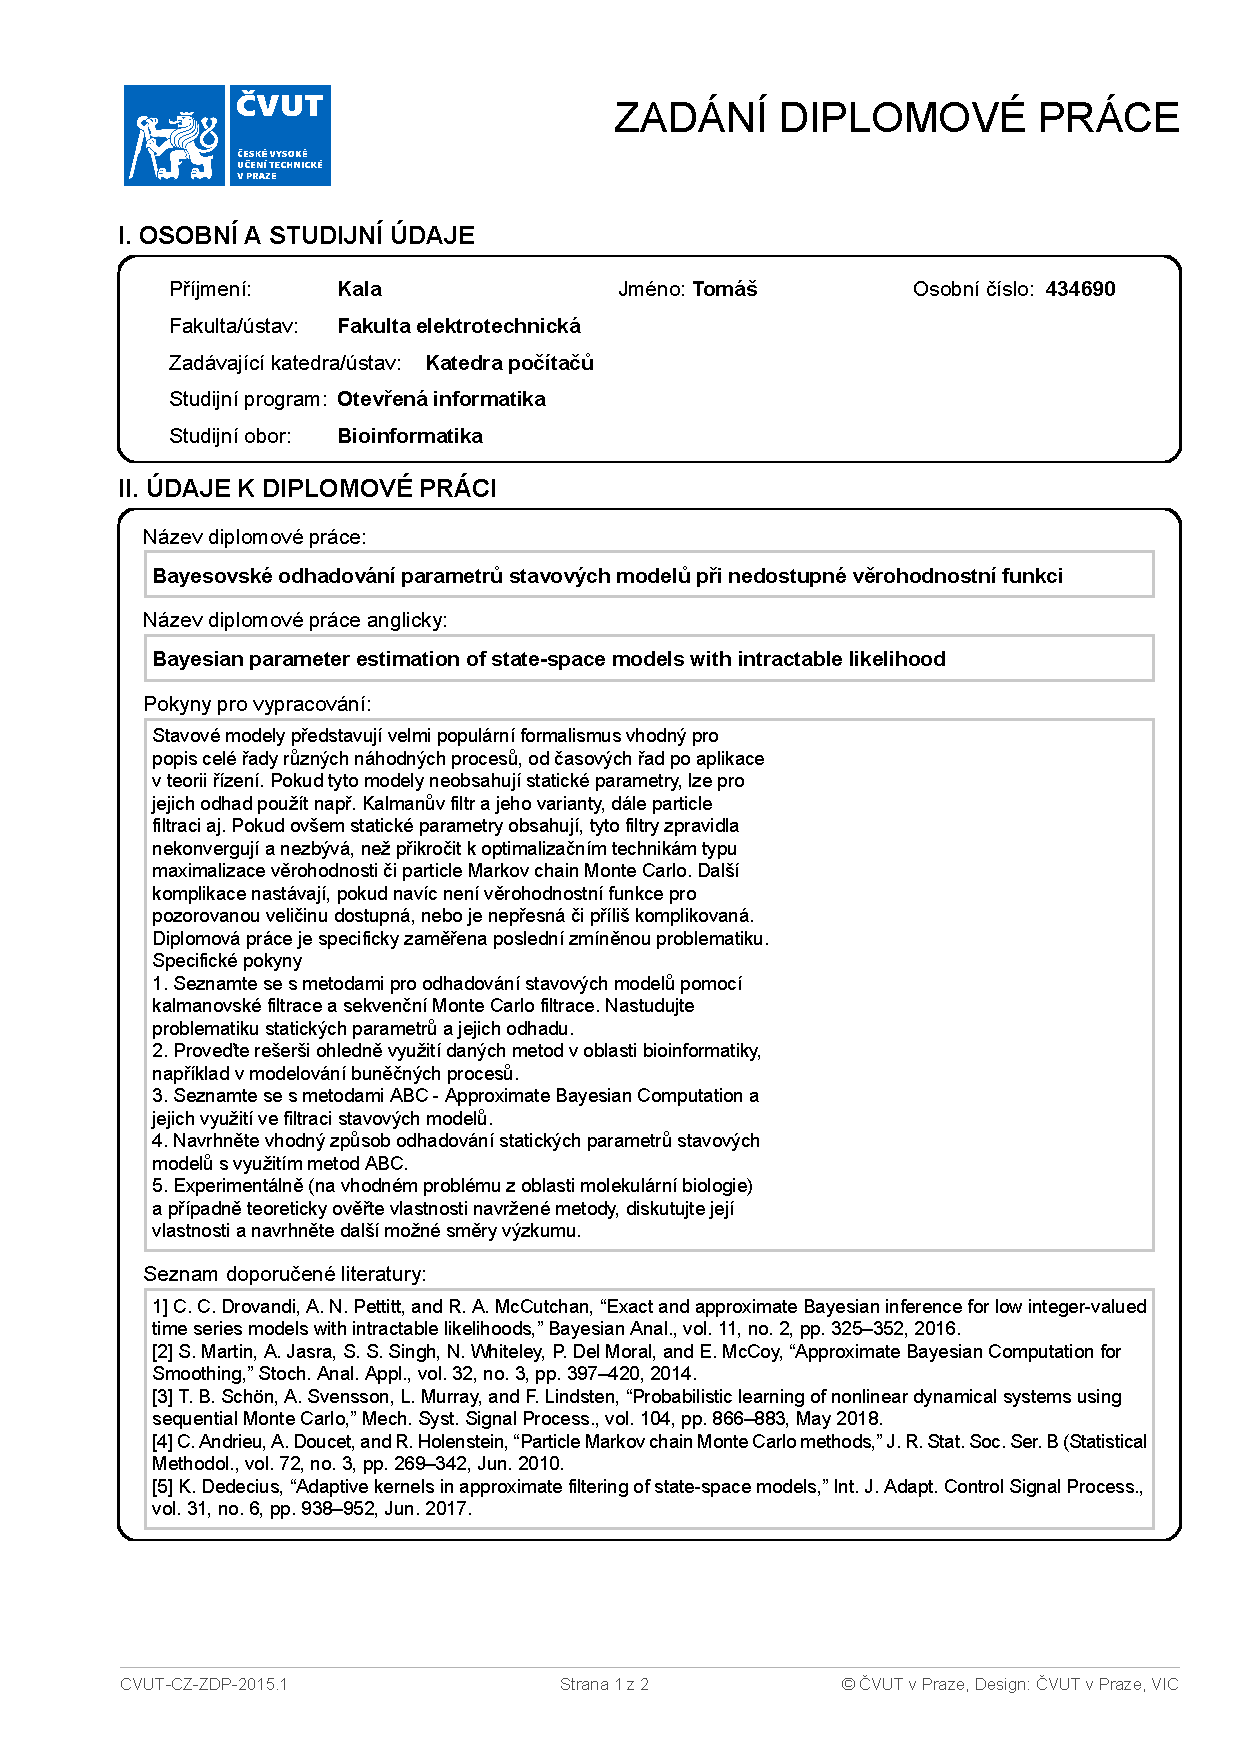
\includepdf[pages=-]{tex/assignment}

% Abstract
\selectlanguage{english}
\cleardoublepage
\begin{abstract}
    State-space models allow for a flexible description of a partially-observed random process, whose transition and observation probability densities depend on a given static parameter. This parameter is either of direct interest, or must be estimated in order to infer about the process latent states. Straightforward inference about the static parameter is typically not possible, since the model likelihood is intractable up to certain special cases. An estimate of this likelihood such that the inference remains correct is then sought. A conventional likelihood estimator utilizes the particle filter, which however requires the observation model to be known. An alternative likelihood estimate not requiring this model to be available is derived through the use of Approximate Bayesian Computation techniques. The developed model is then applied to a molecular biology problem, which describes a simplified prokaryotic auto-regulatory process.
    \newline
    \newline
    \noindent \textbf{Keywords:} State-space model, particle filter, Approximate Bayesian Computation, auto-regulation.
\end{abstract}
\selectlanguage{czech}
\cleardoublepage
\begin{abstract}
    Stavové modely umožňují flexibilní popis částečně pozorovaného náhodného procesu, jehož přechodová pravděpodobnost a model emise závisejí na statickém parametru. Tento parametr je buď přímo středem zájmu, a nebo je nutné ho odhadnout v rámci inference o skrytých stavech modelu. Odhad tohoto statického parametru není snadný, neboť věrohodnost modelu není až na některé speciální případy dostupná. Tuto věrohodnost je tedy nutné odhadnout způsobem, který neovlivní výsledek. Odhad se typicky konstruuje pomocí částicového filtru, který ale vyžaduje přesně určený emisní model procesu. Jako alternativa je odvozen odhad věrohodnosti pomocí metod Approximate Bayesian Computation, které nevyžadují přesně určenou emisní pravděpodobnost. Vyvinutý model je následně aplikován na problém z oblasti molekulární biologie modelující zjednodušený autoregulační proces v prokaryotách.
    \newline
    \newline
    \noindent \textbf{Klíčová slova:} Stavový model, částicový filtr, Approximate Bayesian Computation, autoregulace.
\end{abstract}
\selectlanguage{english}

\chapter*{Author statement for graduate thesis:}

I declare that the presented work was developed independently and that I have listed all sources of information used within it in accordance with the methodical instructions for observing the ethical principles in the preparation of university theses.\\

\noindent Prague, date ........................ \hfill ..........................................
\noindent \begin{flushright}
signature
\end{flushright}
\chapter*{Acknowledgements}

% Table of contents
\tableofcontents

% Chapters
%\cleardoublepage
%\pagenumbering{arabic}

\chapter{Introduction}
\label{chap:introduction}

Probabilistic modelling arises in a wide variety of situations. Often, the measurements one uses to perform inference have been carried out with an unknown error. Frequently, one also does not have access to a correct model for the particular situation --- the true model is either unknown, or such model is even impossible to formulate.

In the former case, one naturally assumes a random error associated with the observations, and attempts to infer something from the data while accounting for this randomness.

In the latter case, one has no choice but to work with a given, although possibly simplified model, purely because of insufficient domain knowledge. Connected with such a model is some degree of uncertainty about its parameters. It is often beneficial to think of these parameters as random variables themselves, in accordance with the Bayesian methodology \citep{bayes}. Such formulation allows to formulate one's prior beliefs about the parameter values, and then updating them upon receiving new observations.

In this thesis, we work with state-space models (SSMs) consisting of a sequence of observed random variables $y_t$ indexed by discrete time $t = 1, \ldots, T$, which have been generated by a latent random process $x_t,\ t = 1, \ldots, T$. The distribution of $x_t$ and $y_t$ is assumed to be parameterized by a static parameter $\theta$. Our goal is to perform posterior inference about this parameter, given a sequence of observations $y_t$. Furthermore, we assume that the likelihood function of the SSM is intractable and must be approximated. This assumption is well-grounded, as the likelihood is only available in severely restricted cases, to be discussed in \autoref{chap:inference}, together with a formal definition of the SSM.

Our contribution is twofold. First, we show how to apply the Approximate Bayesian Computation (ABC) methodology \citep{abc-old-old, abc-old} to obtain an estimate of the likelihood even under a misspecified observation model. Our formulation allows for arbitrary kernel functions with automatically determined widths, unlike the simple accept-reject routine typically discussed in the literature. Second, we apply the resulting model to the genetic auto-regulation process in prokaryotes. Such situation is suitable for a state-space model with a possibly misspecified observation model, as all attempts to model such a complex system are necessarily simplified. To quote the famous statistician George E. P. Box, \emph{``all models are wrong, but some are useful''} \citep{box-quote}. This statement is particularly true for such situations, and it is our hope that our model is indeed useful.

The rest of the thesis is organized as follows:

In \autoref{chap:related-work}, we discuss the related work. First, we review some classical works on Markov Chain Monte Carlo (MCMC) methods. We also discuss how these can be applied to state-space models with an intractable likelihood function. Next, we overview the literature on ABC methods and how these could be used to obtain a suitable likelihood estimate even when the observation model is incorrect. Finally, we discuss the application of related methods in bioinformatics and molecular biology.

In \autoref{chap:inference}, we describe the assumed form of a state-space model. We show how one would implement a sampler to approximately infer the static parameters given a sequence of observations. We also show that in this basic form, such sampler is unusable, since it relies on the evaluation of the likelihood function of the observed sequence, which is intractable (up to certain special cases). We then describe how this likelihood can be estimated using the particle filter \citep{particle-filter} without affecting the asymptotical properties of the sampler.

\autoref{chap:abc} provides a description of the ABC method, and also how it can be applied to estimate the likelihood even under a misspecified model. We discuss the pros and cons of such approach as well as potential issues and how to address them.

\autoref{chap:applications} provides numerical studies, where we apply the model developed in \autoref{chap:abc} to several examples and compare it with the model utilizing the particle filter. This chapter also includes the prokaryotic auto-regulation study discussed earlier.

Finally, \autoref{chap:conclusion} concludes the thesis and discusses some possible directions to be investigated in the future.

\chapter{Related work}
\label{chap:related-work}

In this chapter, we provide a survey of literature relevant to our work. Addressed are works on the use of Markov Chain Monte Carlo methods for approximate inference, works devoted to the use of the particle filter for state-space models likelihood estimation, and those related to Approximate Bayesian Computation methods. The chapter is concluded by a section describing the use of the state-space models in bioinformatics, focusing on problems arising in molecular biology and genetics.

\section{Markov Chain Monte Carlo methods}
Monte Carlo methods can be described as a class of algorithms relying on random sampling to produce numerical results. Typically, the expectation of some transformation of a probability distribution is of interest. This is then approximated by the empirical mean of a transformed random sample generated according to this distribution. Often, the probability distribution of interest is too complex to sample exactly. Assuming that the probability density function of this distribution can be evaluated (at least up to a normalizing constant), Monte Carlo methods are able to output a random sample approximately distributed according to the true distribution. \emph{Markov Chain} Monte Carlo (MCMC) methods employ a Markov chain designed so that its limiting distribution is the target. At least asymptotically, the samples are indeed distributed according to the desired distribution.

An attractive property of MCMC, as opposed to plain Monte Carlo, is that the transition distribution of such chain need not resemble the target distribution even closely, and that the problem is relatively unaffected by the dimensionality. The downside is a difficulty to determine convergence --- for how long should a chain be simulated in order to approximately reach the limiting distribution. In addition, one typically requires independent samples from the target distribution, which, however, the Markov chain samples are \emph{not}. Typically, one needs to ``thin'' the Markov chain samples by keeping every $n$th one to ensure their approximate independence.

Perhaps the best known MCMC algorithm is the Metropolis algorithm \citep{metropolis}, later improved by \cite{hastings}. In this algorithm, random samples are iteratively generated from the Markov chain transition distribution. Each such sample is then compared with the previous one, and accepted with a certain probability ensuring that the limiting distribution is indeed the target. The go-to reference for Monte Carlo methods is \cite{robert-casella}. An appealing treatment of MCMC methods with applications towards physics and machine learning can be found in \cite{information-theory}.

There are of course many more MCMC algorithms. For our task, the Metropolis-Hastings algorithm is sufficient, since the main problem is in the likelihood estimation, and not in designing the best sampler possible.

\section{Parameter inference in state-space models}
We assume that the state-space model (SSM) takes the form informally stated in \autoref{chap:introduction} and more formally given in \autoref{chap:inference}, equation \eqref{eq:factorization}. If all the parameters of interest are changing in time, that is, the inference is about the latent process $\bx_t$ given the observed sample $\by_1, \ldots, \by_T$, one arrives at the task of filtering.

If the transition distribution from state $\bx_t$ to state $\bx_{t+1}$ is linear in the states and corrupted by uncorrelated additive noise centered at 0, this task can be solved exactly by the Kalman filter \citep{kalman}. The resulting filter is then optimal with respect to the mean squared error. An especially nice overview of the Kalman filter connecting it with other linear statistical models is \cite{lds}.

Once the state transition becomes non-linear, as is typically the case, one can use various generalizations of the Kalman filter, such as the extended Kalman filter (EKF), which locally linearizes the transition distribution and then applies the Kalman filter to it, or the unscented Kalman filter \citep{ukf}. These methods come without any optimality guarantees, though. The EKF additionally works best under a very mild non-linearity, due to its first-order approximation.

In recent years, the particle filter \citep{particle-filter} has become a popular alternative due to its simple implementation, appealing asymptotic properties and the fact that it allows for the transition model to be arbitrarily non-linear. Since the particle filter is used later in \autoref{chap:inference}, we postpone a more detailed description there.

If, on the other hand, some of the unknown parameters are static, the task becomes more complex. Blindly applying an MCMC algorithm or any other approximation is not possible, as the likelihood function, on which such algorithms typically depend, cannot be evaluated. The paper \cite{andrieu} introduced the idea of using the particle filter to obtain an estimate of the likelihood, which has been shown by \cite{del-moral} to preserve the limiting distribution of the underlying Markov chain. The resulting algorithm is called \textit{Marginal Metropolis-Hastings}. A more recent overview can be found in the tutorial by \cite{schoen}.

\section{Approximate Bayesian Computation}
In its original formulation, the method of Approximate Bayesian Computation (ABC) provides a way to approximate the posterior distribution $p(\theta \mid y) \propto f(y \mid \theta) p(\theta)$, assuming that the prior $p(\cdot)$ is fully known, and that the likelihood $f(\cdot \mid \theta)$ can be sampled from, but not evaluated \citep{abc-old-old, abc-old}. A more recent treatment of ABC methods can be found in \cite{abc-recent}.

Informally, ABC works by simulating a sample $\tilde{\theta}$ from the prior, substituting it to the likelihood, and generating pseudo-observations $\tilde{y}$. These are then compared to the real observations $y$, and if they are ``similar enough'', the sample $\tilde{\theta}$ is accepted. Otherwise, it is rejected. The posterior distribution of $\theta$ is then given in terms of the accepted samples $\tilde{\theta}$. This variant is referred to as the accept-reject ABC, for obvious reasons.

In this thesis, we apply the ABC method in place of the particle filter to allow for inference about the static parameter $\theta$ when the likelihood is not available. In addition, the use of ABC allows for a possibly misspecified observation model of the SSM, which is often the case, as one may not possess the necessary domain knowledge or computational power needed for the real model. Such a situation has been considered by \cite{jasra-time-series}, although only through the use of the accept-reject variant given above.

Since accepting a sufficient number of samples may take a long time, an idea is to measure the distance between the true and pseudo-observations through a kernel function. This formulation would not reject any samples --- instead, previously rejected samples would get assigned low weights. This has been investigated by \cite{dedecius}, along with a proposed way to automatically tune the kernel width. How to exactly apply the ABC method to our problem is addressed in \autoref{chap:abc} in detail.

\section{Applications to molecular biology}
Finally, we review works describing how the framework of SSMs and their parameter inference can be applied in the context of bioinformatics, focusing on problems of molecular biology and genetics.

The go-to reference for stochastic modelling in biology is \cite{wilkinson-book}. It contains a broad overview of applications of various probabilistic models to examples from molecular biology and chemistry. Included is a description of the Gillespie algorithm \cite{gillespie1, gillespie2} used to simulate chemical reactions, which we use in \autoref{chap:applications}.

A recent application of SSMs to molecular biology can be found in \cite{wilkinson}, where the authors use the particle filter to approximate the unknown likelihoods of various biological models. We implement these examples in \autoref{chap:applications} and compare them with the ABC approximation.

The paper \cite{bio1} models biological networks, such as gene regulatory networks or signalling pathways, by SSMs, and estimates their parameters. The static parameters of the model are viewed as dynamic states which, however, do not change in time. The unscented Kalman filter is then applied to estimate these ``dynamic'' parameters. Such approach is simple, as it does not require the use of MCMC algorithms, but comes without the appealing asymptotic properties of MCMC inference.

\cite{bio2}, \cite{bio3} and \cite{bio4} proceed in a similar fashion when estimating the parameters of various biochemical networks. The used models are only mildly non-linear, and so the extended Kalman filter is sufficient, again without any asymptotic guarantees of identifying the true parameters.

An interesting approach to learning the structure of a gene regulatory network from a gene expression time series can be found in \cite{bio5}. First, the particle filter is applied to learn the hidden states of the network. Once these hidden states are known, the LASSO regression is applied to learn a sparse representation of the regulatory network, since each gene is assumed to interact only with a small number of other genes.
\chapter{Learning the parameters of a state-space model}
\label{chap:inference}

This chapter describes the state-space model (SSM) formulation we are working with. In \autoref{sec:ssm-definition}, we state our assumptions about the individual probability distributions. Then in \autoref{sec:parameter-inference}, we calculate the posterior distribution of the parameters of interest, and show that straightforward inference is not possible. Further on, we derive a sampler to approximate this distribution. By itself, this sampler is unusable, as it requires the evaluation of the model likelihood. To circumvent this, we introduce the particle filter in \autoref{sec:particle-filter}. This section gives the definition and some of the properties of the filter. Later in \autoref{sec:particle-filter-estimate} we show how to use the particle filter to estimate the likelihood, and argue that it does not affect the asymptotic properties of the sampler.

Most of this chapter is based on \cite{andrieu} and \cite{schoen}.



\section{State-Space Model definition} \label{sec:ssm-definition}
The state-space model, often also called the hidden Markov model (HMM) assumes a sequence of latent states $\left\{\bx_t\right\}_{t=0}^\infty \subseteq \R^{d_x}$ following a Markov chain, and a sequence of observed variables $\left\{\by_t\right\}_{t=1}^\infty \subseteq \R^{d_y}$. All involved distributions are parameterized by an unknown static parameter $\btheta \in \Theta \subset \R^d$.

For a fixed time $T \geq 1$, we use the shorthands $\bx_{0:T} = \left\{\bx_t\right\}_{t=0}^T$ and $\by_{1:T} = \left\{\by_t\right\}_{t=1}^T$.

The HMM formulation means that the joint distribution of $\bx_{0:T}$ and $\by_{1:T}$ factorizes, for any $T \geq 1$, into
\begin{equation}\label{eq:factorization}
p(\bx_{0:T}, \by_{1:T} \mid \btheta) = \sprior(\bx_0 \mid \btheta) \prod_{t = 1}^{T} \trans_t(\bx_t \mid \bx_{t-1}, \btheta) \obs_t(\by_t \mid \bx_t, \btheta),
\end{equation}
where $\sprior$ is the prior distribution over the initial state, $\trans_t$ is the transition distribution at time $t$ and $\obs_t$ is the observation model at time $t$.

The factorization \eqref{eq:factorization} can be written more clearly as
\begin{align*}
\bx_0 \mid \btheta & \sim \sprior(\cdot \mid \btheta), \\
\bx_t \mid \bx_{t-1}, \btheta & \sim \trans_t(\cdot \mid \bx_{t-1}, \btheta), \quad t = 1, \ldots, T, \\
\by_t \mid \bx_t, \btheta & \sim \obs_t(\cdot \mid \bx_t, \btheta), \quad t = 1, \ldots, T.
\end{align*}

Finally, in accordance with the Bayesian approach \citep{bayes}, we introduce a prior distribution $\pprior$ over the unknown parameters $\btheta$ quantifying our knowledge about $\btheta$ before observing any data. This allows us to state the full joint distribution
\begin{equation}\label{eq:full-joint}
p(\bx_{0:T}, \by_{1:T}, \btheta) = p(\bx_{0:T}, \by_{1:T} \mid \btheta) \pprior(\btheta).
\end{equation}
The corresponding graphical model is depicted in \autoref{fig:graphical-model}.
\begin{figure}[ht]
    \centering
    \begin{tikzpicture}
    % Style
    \tikzstyle{main}=[circle, minimum size = 10mm, thick, draw =black!80, node distance = 16mm]
    \tikzstyle{connect}=[-latex, thick]
    
    % Nodes X
    \node[main,shape=circle,draw=black](X0) at (1,4) {$\bx_0$};
    \node[main,shape=circle,draw=black](X1) at (3,4) {$\bx_1$};
    \node[main,shape=circle,draw=black](X2) at (5,4) {$\bx_2$};
    \node[](Xdots) at (7,4) {$\ldots$};
    \node[main,shape=circle,draw=black](XT) at (9,4) {$\bx_T$};
    
    % Node theta
    \node[](theta) at (7,2) {$\btheta$};
    
    % Nodes Y
    \node[main,shape=circle,draw=black,fill=black!20](Y1) at (3,0) {$\by_1$};
    \node[main,shape=circle,draw=black,fill=black!20](Y2) at (5,0) {$\by_2$};
    \node[](Ydots) at (7,0) {$\ldots$};
    \node[main,shape=circle,draw=black,fill=black!20](YT) at (9,0) {$\by_T$};

    % Edges XX
    \path [->] (X0) edge[connect] node[left] [above] {$\trans_1$} (X1);
    \path [->] (X1) edge[connect] node[left] [above] {$\trans_2$} (X2);
    \path [->] (X2) edge[connect] node[left] [above] {$\trans_3$} (Xdots);
    \path [->] (Xdots) edge[connect] node[left] [above] {$\trans_T$} (XT);
    
    % Edges XY
    \path [->] (X1) edge[connect] node[left] [left] {$\obs_1$} (Y1);
    \path [->] (X2) edge[connect] node[left] [left] {$\obs_2$} (Y2);
    \path [->] (XT) edge[connect] node[left] [left] {$\obs_T$} (YT);
    
    % Edges theta X
    \path [->] (theta) edge[connect] node[left] {} (X0);
    \path [->] (theta) edge[connect] node[left] {} (X1);
    \path [->] (theta) edge[connect] node[left] {} (X2);
    \path [->] (theta) edge[connect] node[left] {} (XT);
    
    % Edges theta Y
    \path [->] (theta) edge[connect] node[left] {} (Y1);
    \path [->] (theta) edge[connect] node[left] {} (Y2);
    \path [->] (theta) edge[connect] node[left] {} (YT);
    \end{tikzpicture}
    \caption{Graphical model describing the full joint distribution \eqref{eq:full-joint}. The shaded nodes denote the observed variables, white nodes represent the latent variables.}
    \label{fig:graphical-model}
\end{figure}



\section{Parameter inference} \label{sec:parameter-inference}
Given an observed sequence $\by_{1:T}$, Bayesian inference relies on the joint posterior density
\begin{equation}\label{eq:joint-posterior}
p(\btheta, \bx_{0:T} \mid \by_{1:T}) = \underbrace{p(\bx_{0:T} \mid \btheta, \by_{1:T})}_{\text{State inference}} \underbrace{p(\btheta \mid \by_{1:T})}_{\text{Parameter inference}}.
\end{equation}
Our primary interest is to perform inference about the static parameter $\btheta$. From \eqref{eq:joint-posterior}, it is clear that to infer about the hidden states $\bx_{0:T}$, one needs knowledge about $\btheta$, so even if the hidden states are of interest, inference about $\btheta$ is necessary. \autoref{sec:particle-filter-estimate} actually shows how to estimate $\bx_{0:T}$ as a by-product.


\paragraph{Bayesian inference}

To perform Bayesian inference about $\btheta$, we express the posterior of $\btheta$ by applying the Bayes theorem:
\begin{equation*}
p(\btheta \mid \by_{1:T}) = \frac{p(\by_{1:T} \mid \btheta) \pprior(\btheta)}{\int p(\by_{1:T} \mid \btheta) \pprior(\btheta) \dx{\btheta}}.
\end{equation*}

Evaluating the likelihood $p(\by_{1:T} \mid \btheta)$ requires marginalizing over $\bx_{0:T}$:
\begin{equation*}
p(\by_{1:T} \mid \btheta) = \int p(\bx_{0:T}, \by_{1:T} \mid \btheta) \dx{\bx_{0:T}},
\end{equation*}
where $p(\bx_{0:T}, \by_{1:T} \mid \btheta)$ is given in \eqref{eq:factorization}. Unless the SSM is linear and Gaussian, such $d_x(T+1)$-dimensional integral is intractable \citep{andrieu}.


\paragraph{Inference under tractable likelihood assumption}

For the time being, we proceed as if the likelihood was tractable. We derive a sampler for $\btheta$ and note which component cannot be evaluated due to the likelihood being present. \autoref{sec:particle-filter-estimate} then describes the necessary changes to allow circumventing the likelihood evaluation.

Often, the interest is not in the posterior $p(\btheta \mid \by_{1:T})$ itself, but on the expectation of some function $\phi$ w.r.t. this distribution, i.e. on
\begin{equation} \label{eq:posterior-integral}
\E_{p(\btheta \mid \by_{1:T})}[\phi(\btheta)] = \int \phi(\btheta) p(\btheta \mid \by_{1:T}) \dx{\btheta}.
\end{equation}
We use the Metropolis-Hastings algorithm \citep{metropolis, hastings} to obtain $M$ samples from $p(\btheta \mid \by_{1:T})$, denoted as $\btheta^{(m)},\ m = 1, \ldots, M$. The integral \eqref{eq:posterior-integral} is then approximated as the arithmetic mean
\begin{equation*}
\frac{1}{M} \sum_{m=1}^M \phi(\btheta^{(m)}).
\end{equation*}
An appealing property of the Metropolis-Hastings algorithm is that such arithmetic mean converges to \eqref{eq:posterior-integral} almost surely \citep{robert-casella}, i.e.
\begin{equation*}
\frac{1}{M} \sum_{m=1}^M \phi(\btheta^{(m)}) \xrightarrow{a.s} \int \phi(\btheta) p(\btheta \mid \by_{1:T}) \dx{\btheta},
\end{equation*}
where $\xrightarrow{a.s.}$ denotes almost sure convergence.

Finally, we note that if one is indeed interested in the distribution $p(\btheta \mid \by_{1:T})$ itself, it can be recovered by the empirical distribution
\begin{equation*}
\hat{p}(\btheta \mid \by_{1:T}) = \frac{1}{M} \sum_{m=1}^M \delta_{\btheta^{(m)}}(\btheta),
\end{equation*}
where $\delta$ denotes the Dirac distribution. This estimate can be additionally smoothed using kernel methods \citep{kernel-smoothing}.


\paragraph{Metropolis-Hastings algorithm}
The Metropolis-Hastings algorithm is described in \autoref{alg:metropolis-hastings}. Although well-known, it is included for comparison with the variant introduced in \autoref{sec:particle-filter-estimate}.

The target distribution is the parameter posterior $p(\btheta \mid \by_{1:T}) \propto p(\by_{1:T} \mid \btheta) \pprior(\btheta)$. In this case, it is not necessary to evaluate the normalizing constant, since it gets cancelled out.

The algorithm further requires a proposal distribution $\prop$. Similarly to the prior $\pprior$, it is problem-dependent, and must be selected carefully.

\begin{algorithm}[ht]
    \caption{Metropolis-Hastings}
    \label{alg:metropolis-hastings}
    \begin{algorithmic}[1]
        \Input $\text{Number of samples } M,\ \left\{\by_1, \ldots, \by_T\right\}$
        
        \State $\text{Initialize } \btheta^{(0)}.$
        
        \For{$m = 1\ \mathbf{to}\ M$}
            \State $\text{Sample } \btheta^\prime \sim \prop(\cdot \mid \btheta^{(m-1)}).$
            \State $\text{Calculate the aceptance probability } $ \begin{equation} \label{eq:acceptance-probability}
            \alpha = \min \left\{1, \frac{p(\by_{1:T} \mid \btheta^\prime) \pprior(\btheta^\prime)}{p(\by_{1:T} \mid \btheta^{(m-1)}) \pprior(\btheta^{(m-1)})} \frac{\prop(\btheta^{(m-1)} \mid \btheta^\prime)}{\prop(\btheta^\prime \mid \btheta^{(m-1)})} \right\}.
            \end{equation}
            \State $\text{Sample } u \sim \mathcal{U}(0,1).$
            \If {$u \leq \alpha$}
                \State $\btheta^{(m)} \gets \btheta^\prime$ \Comment{With probability $\alpha$, accept the proposed sample.}
            \Else
                \State $\btheta^{(m)} \gets \btheta^{(m-1)}$ \Comment{With probability $1 - \alpha$, reject the proposed sample.}
            \EndIf
        \EndFor
        
        \Output $\left\{ \btheta^{(1)}, \ldots, \btheta^{(M)} \right\}$
    \end{algorithmic}
\end{algorithm}

We see that the acceptance probability \eqref{eq:acceptance-probability} cannot be calculated, as it depends on the intractable likelihood $p(\by_{1:T} \mid \btheta)$. In \autoref{sec:particle-filter-estimate}, we give a modified variant of the Metropolis-Hastings algorithm, where the likelihood is approximated using the particle filter. The derivation of this filter is the content of the next section.



\section{The particle filter} \label{sec:particle-filter}
The particle filter \citep{particle-filter} is a method for approximating the filtering distribution $p(\bx_t \mid \by_{1:t})$ using a finite number of samples called particles. The algorithm is also known as sequential Monte Carlo or sequential importance sampling. The latter name sheds some light on how the method works, and it is exactly through importance sampling that the particle filter is derived.

\paragraph{Importance sampling}
Here we briefly review the basic idea behind importance sampling. For a more thorough treatment, the reader is referred to \cite{information-theory} or \cite{robert-casella}.

Consider a situation where the expectation of some function $\phi$ w.r.t. the distribution with density $p$,
\begin{equation} \label{eq:is-expectation}
\Phi \coloneqq \E_{p}[\phi(\bm{X})] = \int \phi(\bm{x}) p(\bm{x}) \dx{\bm{x}},
\end{equation}
is of interest. Assume that the integral is analytically intractable, and that one cannot generate samples from $p$ to approximate this expectation. Assume further that the density $p$ can be evaluated, at least up to a multiplicative constant, i.e. that it takes the form
\begin{equation*}
p(\bm{x}) = \frac{p^*(\bm{x})}{Z},
\end{equation*}
where $Z$ is an unknown normalizing constant, and $p^*$ can be evaluated. Such situation frequently arises in Bayesian statistics, where a posterior distribution of interest $p(\btheta \mid \bm{x}) = \frac{p(\bm{x} \mid \btheta) p(\btheta)}{\int p(\bm{x} \mid \btheta) p(\btheta) \dx{\btheta}}$ is given in terms of the Bayes theorem. The normalizing constant in the denominator is often unavailable in analytic form. However, the numerator can be evaluated.

Next, we introduce a (typically simpler) distribution with probability density $q(\bm{x}) = \frac{q^*(\bm{x})}{Z_Q}$ such that
\begin{enumerate}
    \item One can sample from $q$;
    \item One can evaluate $q^*$;
    \item $p(\bm{x}) > 0$ implies $q(\bm{x}) > 0$.
\end{enumerate}
The expectation \eqref{eq:is-expectation} can then be written as
\begin{equation*}
\Phi = \int \phi(\bm{x}) \frac{q(\bm{x})}{q(\bm{x})} p(\bm{x}) \dx{\bm{x}} = \int \phi(\bm{x}) \underbrace{\frac{p(\bm{x})}{q(\bm{x})}}_{w^*(\bm{x})} q(\bm{x}) \dx{\bm{x}} = \E_{q}[\phi(\bm{X}) w^*(\bm{X})],
\end{equation*}
where $w^*(\bm{x})$ are called the importance weights. By defining $w(\bm{x}) = \frac{p^*(\bm{x})}{q^*(\bm{x})}$, $\Phi$ can be approximated by
\begin{equation*}
\Phi \approx \widehat{\Phi} \coloneqq \frac{\sum_{i=1}^N \phi(\bm{x}^{(i)}) w(\bm{x}^{(i)})}{\sum_{i=1}^Nw(\bm{x}^{(i)})}, \quad \bm{x}^{(1)}, \ldots, \bm{x}^{(N)} \stackrel{iid}{\sim} q.
\end{equation*}
We note that by using $w$ instead of $w^*$ and normalizing by the weights sum instead of the sample size $N$, we bypass the evaluation of $Z$ and $Z_Q$, since they cancel out. The importance weights here account for correcting the discrepancy between the distribution $q$ and the true distribution $p$.

The estimator $\widehat{\Phi}$ converges to the true expectation $\Phi$ as $N \to \infty$. However, it is not necessarily unbiased \citep{information-theory}.


\paragraph{Sequential importance sampling (SIS)}
The SIS algorithm uses a weighted set of particles $\left\{\left(\bm{x}_t^{(i)}, w_t^{(i)} \right) : i = 1, \ldots, N \right\}$, to represent the filtering distribution $p(\bm{x}_t \mid \by_{1:t})$. To simplify notation, we write $w_t^{(i)}$ instead of $w_t(\bm{x}^{(i)})$ from now on. The empirical approximation to $p(\bm{x}_t \mid \by_{1:t})$ is then
\begin{equation*}
\hat{p}(\bm{x}_t \mid \by_{1:t}) = \frac{\sum_{i=1}^N w_t^{(i)} \delta_{\bm{x}_t^{(i)}}(\bm{x}_t)}{\sum_{i=1}^N w_t^{(i)}}.
\end{equation*}

As the name suggests, the algorithm involves a sequential application of the importance sampling procedure with increasing time $t$.

Returning to the SSM \eqref{sec:ssm-definition}, we consider the posterior distribution of a sequence of states $\bx_{0:t}$ given a sequence of observations $\by_{1:t}$. By application of the Bayes theorem, we obtain the following recursive formula:
\begin{equation*}
\begin{split}
p(\bx_{0:t} \mid \by_{1:t}) & \propto p(\by_t \mid \bx_{0:t}, \by_{1:t-1}) p(\bx_{0:t} \mid \by_{1:t-1}) \\
&= \obs_t(\by_t \mid \bx_t) p(\bx_t \mid \bx_{0:t-1}, \by_{1:t-1}) p(\bx_{0:t-1} \mid \by_{1:t-1}) \\
&= \obs_t(\by_t \mid \bx_t) \trans_t(\bx_t \mid \bx_{t-1}) p(\bx_{0:t-1} \mid \by_{1:t-1}),
\end{split}
\end{equation*}
where the equalities follow from the hidden Markov model independence assumptions.

For the target $p(\bx_{0:t} \mid \by_{1:t})$, we introduce the importance sampling distribution $q(\bx_{0:t} \mid \by_{1:t})$ and sample $\bx_{0:t}^{(i)}$ from it. The importance weights are (up to normalization) given by
\begin{equation} \label{eq:weight-recursion1}
\begin{split}
w_t^{(i)} & \propto \frac{p(\bx_{0:t}{(i)} \mid \by_{1:t})}{q(\bx_{0:t}^{(i)} \mid \by_{1:t})} \\
& \propto \frac{\obs_t(\by_t \mid \bx_t^{(i)}) \trans_t(\bx_t^{(i)} \mid \bx_{t-1}^{(i)}) p(\bx_{0:t-1}^{(i)} \mid \by_{1:t-1})}{q(\bx_{0:t}^{(i)} \mid \by_{1:t})}.
\end{split}
\end{equation}
By definition of the conditional probability and the hidden Markov model assumptions, we can write the importance sampling distribution as
\begin{equation*}
q(\bx_{0:t} \mid \by_{1:t}) = q(\bx_t \mid \bx_{0:t-1}, \by_{1:t}) q(\bx_{0:t-1} \mid \by_{1:t-1}).
\end{equation*}
By substituting into \eqref{eq:weight-recursion1}, we obtain the following recursion:
\begin{equation} \label{eq:weight-recursion2}
\begin{split}
w_t^{(i)} & \propto \frac{\obs_t(\by_t \mid \bx_t^{(i)}) \trans_t(\bx_t^{(i)} \mid \bx_{t-1}^{(i)})}{q(\bx_t^{(i)} \mid \bx_{0:t-1}^{(i)}, \by_{1:t})} \frac{p(\bx_{0:t-1}^{(i)} \mid \by_{1:t-1})}{q(\bx_{0:t-1}^{(i)} \mid \by_{1:t-1})} \\
& \propto \frac{\obs_t(\by_t \mid \bx_t^{(i)}) \trans_t(\bx_t^{(i)} \mid \bx_{t-1}^{(i)})}{q(\bx_t^{(i)} \mid \bx_{0:t-1}^{(i)}, \by_{1:t})} w_{t-1}^{(i)}.
\end{split}
\end{equation}
So updating the $i$th weight when transitioning from time $t-1$ to $t$ is a relatively simple task involving only multiplication by the first fraction in \eqref{eq:weight-recursion2}.

The sequential importance sampling algorithm is summarized in \autoref{alg:sis}.
\begin{algorithm}[ht]
    \caption{Sequential Importance Sampling}
    \label{alg:sis}
    \begin{algorithmic}[1]
        \Input $\text{Number of particles } N,\ \text{current parameter value } \btheta,\ \left\{\by_1, \ldots, \by_T\right\}$
        
        \State $\text{Sample } \bx_0^{(i)} \sim \sprior(\cdot \mid \btheta), \quad i = 1, \ldots, N.$ \Comment{Initialize $N$ particles.}
        
        \State $w_0^{(i)} \gets \frac{1}{N}, \quad i = 1, \ldots, N.$ \Comment{Initialize uniform weights.}
        
        \For{$t = 1\ \mathbf{to}\ T$}
            \State $\text{Sample } \bx_t^{(i)} \sim q(\cdot \mid \bx_{0:t-1}^{(i)}, \by_{1:t}), \quad i = 1, \ldots, N.$ \Comment{Sample $N$ new particles.}
            \State $w_t^{(i)} \propto \frac{\obs_t(\by_t \mid \bx_t^{(i)}) \trans_t(\bx_t^{(i)} \mid \bx_{t-1}^{(i)})}{q(\bx_t^{(i)} \mid \bx_{0:t-1}^{(i)}, \by_{1:t})} w_{t-1}^{(i)}$ \Comment{Update the importance weights as per \eqref{eq:weight-recursion2}.}
        \EndFor
    \end{algorithmic}
\end{algorithm}
This by itself is almost the particle filter. There are still two issues to be addressed, though. First, the problem of weight degeneracy discussed in the next paragraph. Second, the choice of the importance sampling distribution $q$ addressed later.


\paragraph{Resampling}
A serious problem preventing the use of the SIS algorithm is that the weights degenerate over time. In each time step, the variance of the weights reduces \citep{particle-filter}. This means that the (normalized) weights always converge to a situation where a single weight is 1 and the others are 0.

To alleviate this, the following resampling step is introduced.
\begin{algorithm}[ht]
    \caption{Multinomial resampling}
    \label{alg:resampling}
    \begin{algorithmic}[1]
        \Input $\text{Importance weights } w_t^{(1)}, \ldots, w_t^{(N)},\ \text{particles } \bx_t^{(1)}, \ldots, \bx_t^{(N)}.$
        
        \State $\widetilde{w}_t^{(i)} \gets \frac{w_t^{(i)}}{\sum_{j=1}^N w_t^{(j)}}, \quad i = 1, \ldots, N.$ \Comment{Normalize the weights.}
        
        \State $\text{Sample } a_i \sim \text{Mult}_N \left(1, \left(\widetilde{w}_t^{(1)}, \ldots, \widetilde{w}_t^{(N)}\right) \right), \quad i = 1, \ldots, N.$ \Comment{Sample indices with replacement.}
        
        \State $w_t^{(a_i)} \gets \frac{1}{N}, \quad i = 1, \ldots, N.$ \Comment{Reset weights.}
        
        \Output $\text{Resampled particles } \bx_t^{(a_1)}, \ldots, \bx_t^{(a_N)} \text{ and weights } w_t^{(a_1)}, \ldots, w_t^{(a_N)}.$
    \end{algorithmic}
\end{algorithm}

The normalized importance weights are interpreted as a probability vector of a categorical distribution. The particles are then resampled (sampled with replacement) according to this distribution. This effectively selects a population of ``strong individuals'' for the next time step.

The above described procedure is known as the multinomial resampling. There are other, more complex, approaches, such as the stratified resampling \citep{resampling}. For our purposes, the multinomial resampling is sufficient.

\paragraph{The particle filter}
The remaining step is the choice of the importance sampling distribution $q$. Obviously, the more similar this distribution is to the target, the closer approximation we obtain.

With the SSM model \eqref{eq:factorization}, it is actually possible to use the target distribution.

{\color{red} TODO}

The resulting algorithm is then called the bootstrap particle filter, due to the resampling step effectively performing a non-parametric bootstrap {\color{red} TODO: Cite bootstrap?}.



\section{Using the particle filter to estimate the likelihood} \label{sec:particle-filter-estimate}
\chapter{Approximate Bayesian Computation}
\label{chap:abc}

We are now in possession of a sampler able to approximate the posterior distribution $p(\btheta \mid \by_{1:T})$ even when the model likelihood is not tractable. As such, the sampler can be used in general non-linear SSMs, as long as the observation model $\obs_t(\by_t \mid \bx_t, \btheta)$ is a well-defined probability density. This requirement can be relaxed by introducing the method of Approximate Bayesian Computation (ABC). The algorithm derived in this chapter utilizes the ABC framework to approximate the SSM likelihood even when the observation model is misspecified or given only as a deterministic mapping $\bx_t \mapsto \by_t$. This allows to infer $\btheta$ even when $\obs_t(\by_t \mid \bx_t, \btheta)$ is not given in terms of a probability density function.

We first motivate the use of ABC methods in our problem in \autoref{sec:abc-motivation}. Then, in \autoref{sec:abc-general}, we describe the method in general and discuss some limitations. \autoref{sec:abc-ssm} introduces ABC to our state-space model framework and addresses some potential issues through kernel functions. Finally, in \autoref{sec:abcmh}, we summarize how exactly is the ABC method used in our model, and provide an alternative variant of the Metropolis-Hastings algorithm which relies on ABC instead of the particle filter to estimate the likelihood.


\section{Motivation} \label{sec:abc-motivation}
In the previous chapter, we derived a way to bypass the likelihood function evaluation when calculating the Metropolis-Hastings acceptance ratio. The method relies on the particle filter to calculate a set of weights $w_t^{(i)} \propto \obs_t(\by_t \mid \bx_t^{(i)}, \btheta)$, where $\obs_t(\by_t \mid \bx_t^{(i)}, \btheta)$ is the observation model defined in \eqref{eq:factorization}. These weights are used to estimate the likelihood $p(\by_{1:T} \mid \btheta)$ as given in \eqref{eq:likelihood-estimate}. However, calculating the weights in such way requires full knowledge of this observation model.

In practice, one may not have access to a correct observation model in the form of a probability density $\obs_t(\by_t \mid \bx_t, \btheta)$. Instead, only a model of the process which generates an observation $\by_t$ from the latent state $\bx_t$ may be available. This generative process may take the form of a differential equation, chemical reaction, simulation, etc. One is then in possession of a mean to generate an observation, but not to evaluate how probable it is. By attempting to fit an arbitrary probability distribution to this generative model, an error is necessarily introduced. The particle filter weights might then not reflect reality, and would lead to incorrect results when using such misspecified model for $\obs_t(\by_t \mid \bx_t, \btheta)$.

As an alternative way to approximate the likelihood ${p(\by_{1:T} \mid \btheta)}$, we can utilize our knowledge of the generative process $\bx_t \mapsto \by_t$ to simulate a number of pseudo-observations $\bu_t$. A surrogate for the observation density $\obs_t(\by_t \mid \bx_t, \btheta)$ is then calculated by evaluating the closeness of these pseudo-observations to the true measurement $\by_t$. Intuitively, if a large number of the simulated observations fall close to $\by_t$, we would expect the true probability density to be high in that region. By bypassing the evaluation of $\obs_t(\by_t \mid \bx_t, \btheta)$, inference can proceed even without knowing the observation model density. This is exactly the idea behind the approximate Bayesian computation methodology; it is discussed in \autoref{sec:abc-general}.

Unfortunately, such approximation comes at a price. In \autoref{chap:inference}, it has been shown that using the particle filter does not introduce any approximation error, since the likelihood estimate is unbiased and leaves the limiting distribution of the Metropolis-Hastings Markov chain intact. This is not the case when applying ABC methods, see \autoref{sec:abc-ssm}.


\section{ABC in general} \label{sec:abc-general}
Before describing how to apply ABC to state-space models, we first summarize the underlying ideas. The ABC method is introduced in the context of general Bayesian inference under a misspecified likelihood function. Later on, we build on these foundations when applying ABC to our SSM framework.

One thing to note is that ABC has traditionally been applied to estimate the posterior $p(\btheta \mid \by)$ for some parameter $\btheta$ and observation $\by$. The method is first considered with this application in mind, and in \autoref{sec:abc-ssm}, we describe how use it to estimate the SSM likelihood instead.

\paragraph{Approximate Bayesian Computation}
The methodology of ABC dates back to \cite{abc-old-old}, where a procedure using simulated psedudo-observations to approximate the posterior distribution was first described. Lately, ABC methods have gained popularity in modelling biological processes \citep{abc-old}. A more recent review can be found in \cite{abc-recent, abc-super-recent}.

In its classical formulation, ABC provides a way to approximate an intractable posterior ${p(\btheta \mid \by) \propto p(\by \mid \btheta) \pprior(\btheta)}$ by introducing an auxiliary variable $\bu$. The posterior approximation is then constructed by integrating over this variable and considering only values sufficiently close to the true measurement \citep{jasra-filtering}. It takes the form of
\begin{equation} \label{eq:abc-integral}
p(\btheta \mid \by) \approx p^\epsilon(\btheta \mid \by) = \frac{\int \I_{\A_{\epsilon, \by}}(\bu) p(\bu \mid \btheta) \pprior(\btheta) \; \dx{\bu}}{\int_{\A_{\epsilon, \by}} \dx{\bu}},
\end{equation}
where $\I_{\A_{\epsilon, \by}}$ is the indicator function of a set $\A_{\epsilon, \by} = \left\{\bu \in \R^{d_y} : \rho(\bu, \by) \leq \epsilon \right\}$ and $\rho: \R^{d_y} \times \R^{d_y} \to \R$ is a metric, typically the Euclidean distance.

The motivation behind \eqref{eq:abc-integral} is that such integral can be approximated by randomly sampling from the likelihood $p(\cdot \mid \btheta)$ without needing to evaluate it. This way, the likelihood can exist only conceptually, and we are able to simulate samples $\bu$ from a model reflecting some real-world process, without considering the underlying probability density.

The hyper-parameter $\epsilon \geq 0$ controls how far the auxiliary variable $\bu$ can be from the true measurement $\by$ to be considered similar. Clearly, if we set $\epsilon = 0$, the integral becomes $p(\by \mid \btheta) \pprior(\btheta)$, and we recover the true posterior. In general, the smaller $\epsilon$, the better approximation is obtained, though at the cost of increased computational complexity.

To avoid the curse of dimensionality, a summary statistic $\bm{s}: \R^{d_y} \to \R^p$, $1 \leq p < d_y$ is often introduced. Instead of comparing $\rho(\bu, \by) \leq \epsilon$, one then compares $\rho(\bm{s}(\bu), \bm{s}(\by)) \leq \epsilon$ (assuming that the metric has been redefined to $\rho: \R^p \times \R^p \to \R$).

It can be shown that if $\bm{s}$ is a sufficient statistic for the parameter $\btheta$, the probability density $p^\epsilon(\btheta \mid \by)$ converges to $p(\btheta \mid \by)$ as $\epsilon \to 0$ \citep{jasra-time-series}. However, it is typically impossible to find such statistic outside of the exponential family of distributions. Otherwise, using a statistic that is not sufficient introduces an additional approximation error.

\paragraph{Basic version of the ABC simulation}
We now give a basic variant of a sampling-based approximation to $p^\epsilon(\btheta \mid \by)$. In the spirit of \eqref{eq:abc-integral}, \autoref{alg:abc-rejection} performs rejection sampling by comparing whether a sampled $\bu$ is in $\A_{\epsilon, \by}$ or not. After describing the algorithm, we discuss some limitations of this basic approach.
\begin{algorithm}[ht]
    \caption{ABC Rejection Algorithm}
    \label{alg:abc-rejection}
    \begin{algorithmic}[1]
        \Input $\text{Number of samples } M, \text{ observation } \by, \text{ metric } \rho, \text{ maximum distance } \epsilon.$
        
        \State $i \gets 1$
        
        \While{$i \leq M$}
        \State $\text{Sample } \btheta^\prime \sim \pprior(\cdot).$ \Comment{Sample from the prior.}
        \State $\text{Simulate } \bu \text{ from } p(\cdot \mid \btheta^\prime).$ \Comment{Simulate a pseudo-observation.}
        
        \If {$\rho(\bu, \by) \leq \epsilon$}
        \State $\btheta^{(i)} \gets \btheta^\prime$ \Comment{Accept the proposed sample.}
        \State $i \gets i + 1$
        \EndIf
        \EndWhile
        
        \Output $\text{Accepted samples } \left\{ \btheta^{(1)}, \ldots, \btheta^{(M)} \right\}.$
    \end{algorithmic}
\end{algorithm}

ABC rejection iteratively samples parameters $\btheta^\prime$ from the prior, plugs them into the likelihood $p(\cdot \mid \btheta^\prime)$, and simulates pseudo-observations $\bu$. These are then compared to the true measurement $\by$ using the metric $\rho$. If the proposed parameter $\btheta^\prime$ gave rise to a pseudo-observation similar enough to the true $\by$ (i.e., $\bu \in \A_{\epsilon, \by}$), the parameter is kept under the assumption that the true data are likely under $\btheta^\prime$. The ABC approximation is then given in terms of the accepted samples $\btheta^{(1)}, \ldots, \btheta^{(M)}$ as the empirical distribution
\begin{equation*}
p(\btheta \mid \by) \approx \frac{1}{M} \sum_{i=1}^M \delta_{\btheta^{(i)}}(\btheta).
\end{equation*}

Setting a low value of $\epsilon$ increases the approximation accuracy, at the cost of increased rejection rate. On the other hand, setting $\epsilon$ too large causes the algorithm to accept more often, but leads to simulating pseudo-measurements dissimilar to $\by$ and, in turn, incorrect $\btheta^{(i)}$. Setting a suitable value of $\epsilon$ is therefore the main difficulty when using ABC. Several approaches are discussed by \cite{jasra-filtering, jasra-time-series}. One particular way \citep{dedecius} is used in \autoref{sec:abc-ssm} in the context of SSMs.

There are many improvement to the basic ABC of \autoref{alg:abc-rejection}, discussed for instance by \cite{abc-recent}. In particular, more sophisticated sampling approaches relying again on MCMC are described. This is not an issue relevant to the SSM framework, as the samples are generated in a different fashion, given in the next section.

\section{ABC in SSMs} \label{sec:abc-ssm}
Next, we describe how exactly is the ABC methodology applied in the context of SSMs.

\autoref{sec:abc-general} states that the typical use case of ABC arises in cases where we have knowledge about the data-generating process, but are unable to evaluate the probability of such data. In the context of SSMs, this translates into knowing how the observed values $\by_t$ have been generated from the latent states $\bx_t$, but being unable to evaluate the density $\obs_t(\by_t \mid \bx_t, \btheta)$. This prevents us from calculating the importance weights $w_t$ through the particle filter, which relies on the availability of $\obs_t(\by_t \mid \bx_t, \btheta)$.

\cite{tina-toni} and \cite{jasra-filtering} describe how a filter could be constructed using the ABC approximation. Additionally, \cite{jasra-time-series} applies this filter in the context of SSMs. We first discuss the construction of this filter. Afterwards, we address a particular limitation of this approach through kernel functions.

\paragraph{Filter construction through ABC}
In SSMs, the dimensionality of the observation space is typically low; the observations are often scalar quantities. It is then not necessary to consider any summary statistics.

\cite{jasra-filtering} consider a modification of the particle filter (\autoref{alg:particle-filter}) which simulates pseudo-observations according to the observation model, and calculates the importance weights based on their closeness to the true measurements. The pseudocode is given in \autoref{alg:abc-filter}.

\begin{algorithm}[ht]
    \caption{ABC-based filter}
    \label{alg:abc-filter}
    \begin{algorithmic}[1]
        \Input $\text{Number of particles } N,\ \text{current parameter value } \btheta, \text{maximum distance } \epsilon,\ \left\{\by_1, \ldots, \by_T\right\}.$
        
        \State $\text{Sample } \bx_0^{(i)} \sim \sprior(\bx_0 \mid \btheta), \quad i = 1, \ldots, N.$ \Comment{Initialize $N$ particles.}
        
        \State $w_0^{(i)} \gets \frac{1}{N}, \quad i = 1, \ldots, N.$ \Comment{Initialize uniform weights.}
        
        \For{$t = 1\ \mathbf{to}\ T$}
        \State $\text{Sample } \bx_t^{(i)} \sim \trans_t(\bx_t \mid \bx_{t-1}^{(i)}, \btheta), \quad i = 1, \ldots, N.$ \Comment{Sample $N$ new particles.}
        
        \State $\text{Simulate } \bu_t^{(i)} \text{ from } \obs_t(\bu_t \mid \bx_t^{(i)}, \btheta), \quad i = 1, \ldots, N.$ \Comment{Simulate $N$ pseudo-observations.}
        
        \State $\text{Set } w_t^{(i)} \propto \I_{\A_{\epsilon, \by_t}}(\bu_t^{(i)}) w_{t-1}^{(i)}, \quad i = 1, \ldots, N.$
        
        \State $\text{Resample } \bx_t^{(i)} \text{ and reset } w_t^{(i)} \text{ using \autoref{alg:resampling}}, \quad i = 1, \ldots, N.$
        \EndFor
    \end{algorithmic}
\end{algorithm}

The algorithm proceeds similarly to \autoref{alg:particle-filter} except for the way the weights are computed. Instead of evaluating the unavailable density $\obs_t(\by_t \mid \bx_t, \btheta)$ at the true observation $\by_t$, a pseudo-observation $\bu_t$ is simulated. The weight is then set to a non-zero value if ${\bu_t \in \A_{\epsilon, \by_t}}$, and 0 otherwise. It may seem that the weights for the same particle $i$ necessarily collapse to 0 after a number of time steps due to the recursive multiplication in step 6. However, step 7 resets the weights uniformly after resampling, so such collapse does not occur.

Analogously to \autoref{sec:particle-filter-estimate}, the weights are then used to approximate the likelihood $p(\by_{1:T} \mid \btheta)$. According to \cite{jasra-time-series}, the estimate is given by
\begin{equation} \label{eq:abc-likelihood}
\widehat{\aux} = \prod_{t=1}^T \frac{1}{N} \sum_{i=1}^N \frac{w_t^{(i)}}{\int_{\A_{\epsilon, \by_t}} \dx{\bu}}.
\end{equation}
The integral in the denominator essentially normalizes the weights $w_t^{(i)}$ to be equal to the probability density of $\mathcal{U}(\by_t; \epsilon)$, the uniform distribution in a sphere centered at $\by_t$ with radius $\epsilon$ given in terms of the metric $\rho$.

\paragraph{Bias}
The use of this ABC filter introduces bias to the parameter inference. Recall that in \autoref{sec:particle-filter-estimate}, we required $\widehat{\aux}$ to be an unbiased estimator of $p(\by_{1:T} \mid \btheta)$. This was the case when the weights were calculated according to $w_t^{(i)} \propto \obs_t(\by_t \mid \bx_t) w_{t-1}^{(i)}$. This unbiasedness is not preserved here, since $\widehat{\aux}$ estimates
\begin{equation*}
\begin{split}
p^\epsilon(\by_{1:T} \mid \btheta) &= \int p^\epsilon(\bx_{0:T}, \by_{1:T} \mid \btheta) \; \dx{\bx_{0:T}} \\
&= \int \sprior(\bx_0 \mid \btheta) \prod_{t=1}^T \trans_t(\bx_t \mid \bx_{t-1}, \btheta) \obs_t^\epsilon(\by_t \mid \bx_t, \btheta) \; \dx{\bx_{0:T}}
\end{split}
\end{equation*}
(compare the inside of the integral with \eqref{eq:factorization}), as noted by \cite{jasra-time-series}. Here the approximate observation density is given by the ABC form
\begin{equation*}
\obs_t^\epsilon(\by_t \mid \bx_t, \btheta) = \frac{\int \I_{\A_{\epsilon, \by_t}}(\bu) \obs_t(\bu \mid \bx_t, \btheta) \; \dx{\bu}}{\int_{\A_{\epsilon, \by_t}} \dx{\bu}},
\end{equation*}
similarly to \eqref{eq:abc-integral}. This essentially means that by plugging \eqref{eq:abc-likelihood} into the Metropolis-Hastings acceptance ratio, the limiting distribution of the underlying Markov chain becomes $p^\epsilon(\btheta \mid \by_{1:T}) \propto p^\epsilon(\by_{1:T} \mid \btheta) \pprior(\btheta)$, instead of the correct $p(\btheta \mid \by_{1:T})$. In general, this bias cannot be dealt with, and is a price to pay for using the incorrect observation model.

An interesting way to address this deficiency has been proposed by \cite{noisy-abc1} and by \cite{noisy-abc2}. The authors note that one uses data $\by_{1:T}$ assumed to have been generated according to \eqref{eq:factorization}, $p(\by_{1:T} \mid \btheta)$, but fitting the ABC approximation $p^\epsilon(\by_{1:T} \mid \btheta)$. In an attempt to bring the data closer the model being really fitted, the authors use a sequence of perturbed observations $\bm{z}_t = \by_t + \bm{v}$, $\bm{v} \sim \mathcal{U}(\bm{0}; \epsilon)$ which denotes the uniform distribution in a sphere given by $\rho$, with radius $\epsilon$ and centered at the origin. It is proved that if $\btheta$ is estimated according to maximum likelihood, the estimate is consistent when using the perturbed sequence $\bm{z}_{1:T}$. This approach is called the Noisy ABC.


\paragraph{Use of kernel functions}
A limitation of \autoref{alg:abc-rejection} and \autoref{alg:abc-filter} lies in the use of the indicator function $\I_{\A_{\epsilon, \by}}$. There are two problems:
\begin{enumerate}
    \item A practical one; it may happen that no samples are accepted and the output is null in the case of \autoref{alg:abc-rejection}, or too many weights become zero in the case of \autoref{alg:abc-filter} and the filter collapses.
    \item A more fundamental one, the simulated pseudo-observations $\bu_t$ are all assigned equal weights, regardless of how far they lie from the true measurement $\by_t$. Intuitively, a pseudo-observation closer to the true $\by_t$ should be assigned a higher weight than one which is further away.
\end{enumerate}
Both issues can be mitigated by considering a general kernel function in place of the indicator $\I_{\A_{\epsilon, \by}}$. Let a kernel of width $\epsilon$ centered at $\by$ and evaluated at $\bu$ be denoted by $\kappa(\bu; \by, \epsilon)$. In machine learning, kernel functions are often taken \emph{proportional} to some symmetric probability density function \citep{elements}. However, as we aim to replace the indicator function $\I_{\A_{\epsilon, \by}}$ by such kernel, we require the kernel to be properly normalized (integrate to unity) to mirror the normalization in \eqref{eq:abc-likelihood}.

With the kernel function, we can write $w_t^{(i)} \propto \kappa(\bu_t; \by_t, \epsilon) w_{t-1}^{(i)}$. The likelihood estimate \eqref{eq:abc-likelihood} becomes
\begin{equation} \label{eq:abc-likelihood-kernel}
\widehat{\aux} = \prod_{t=1}^T \frac{1}{N} \sum_{i=1}^N w_t^{(i)}
\end{equation}
due to the kernel being normalized. This way, the weights are no longer uniform but reflect the distance of $\bu_t$ from $\by_t$. There is also no risk of the filter collapsing due to majority of the weights becoming zero.

Introducing the kernel function to the weights computation is in principle similar to using importance sampling rather than simple rejection sampling \citep{information-theory}. Instead of accepting/rejecting the generated samples based on whether they match some criterion, they are all accepted and weighted according to \emph{how well} they match it.

With the kernel functions in mind, we describe a procedure for automatic tuning of the kernel width $\epsilon$, which has been ignored so far. The adopted method has been derived in a one-dimensional setting, i.e., $\bu, \by \in \R$. We correspondingly denote $\by$ by $y$ and $\bu$ by $u$. When considering multivariate observations, the kernels are applied coordinate-wise (assuming independence between the components of $\by$ or $\bu$, respectively).

Before describing the kernel tuning procedure, we give several examples of commonly used kernel functions and comment on their usage. The kernels are shown in \autoref{fig:kernels}.
\begin{enumerate}
    \item \textbf{Gaussian kernel} The Gaussian kernel takes the form
    \begin{equation*}
    \kappa(u; y, \epsilon) = \frac{1}{\sqrt{2 \pi \epsilon^2}} \exp \left\{-\frac{\left(u - y\right)^2}{2 \epsilon^2}\right\}.
    \end{equation*}
    It is one of the most-commonly used kernel functions.
    \item \textbf{Cauchy  kernel} The Cauchy kernel takes the form
    \begin{equation*}
    \kappa(u; y, \epsilon) = \frac{1}{\pi \epsilon \left[ 1 + \left(\frac{u - y}{\epsilon}\right)^2 \right]}.
    \end{equation*}
    As opposed to the Gaussian distribution, the Cauchy distribution has heavier tails, which make it suitable for situations with potentially distant observations. This kernel typically assigns non-trivial probability even to distant pseudo-observations, preventing the filter from collapsing under outliers.
    
    \item \textbf{Uniform kernel} The uniform kernel takes the form
    \begin{equation*}
    \kappa(u; y, \epsilon) = \begin{cases}
    \frac{1}{2 \epsilon}, & y - \epsilon < u < y + \epsilon; \\
    0, & \text{otherwise}.
    \end{cases}
    \end{equation*}
    Using this kernel, we recover the standard ABC which accepts $u$ if $u \in \A_{\epsilon, y} = \left\{u : \left| u - y \right| < \epsilon \right\}$. If we are in a situation with multivariate observations $\by_t$ and apply the uniform kernel coordinate-wise, the set of accepted samples coincides with the standard ABC using $\rho(\bu, \by) = \max_{i=1}^{d_y} \left|u_i - y_i\right|$, the $L_\infty$ distance.
\end{enumerate}

\begin{figure}[ht]
    \centering
    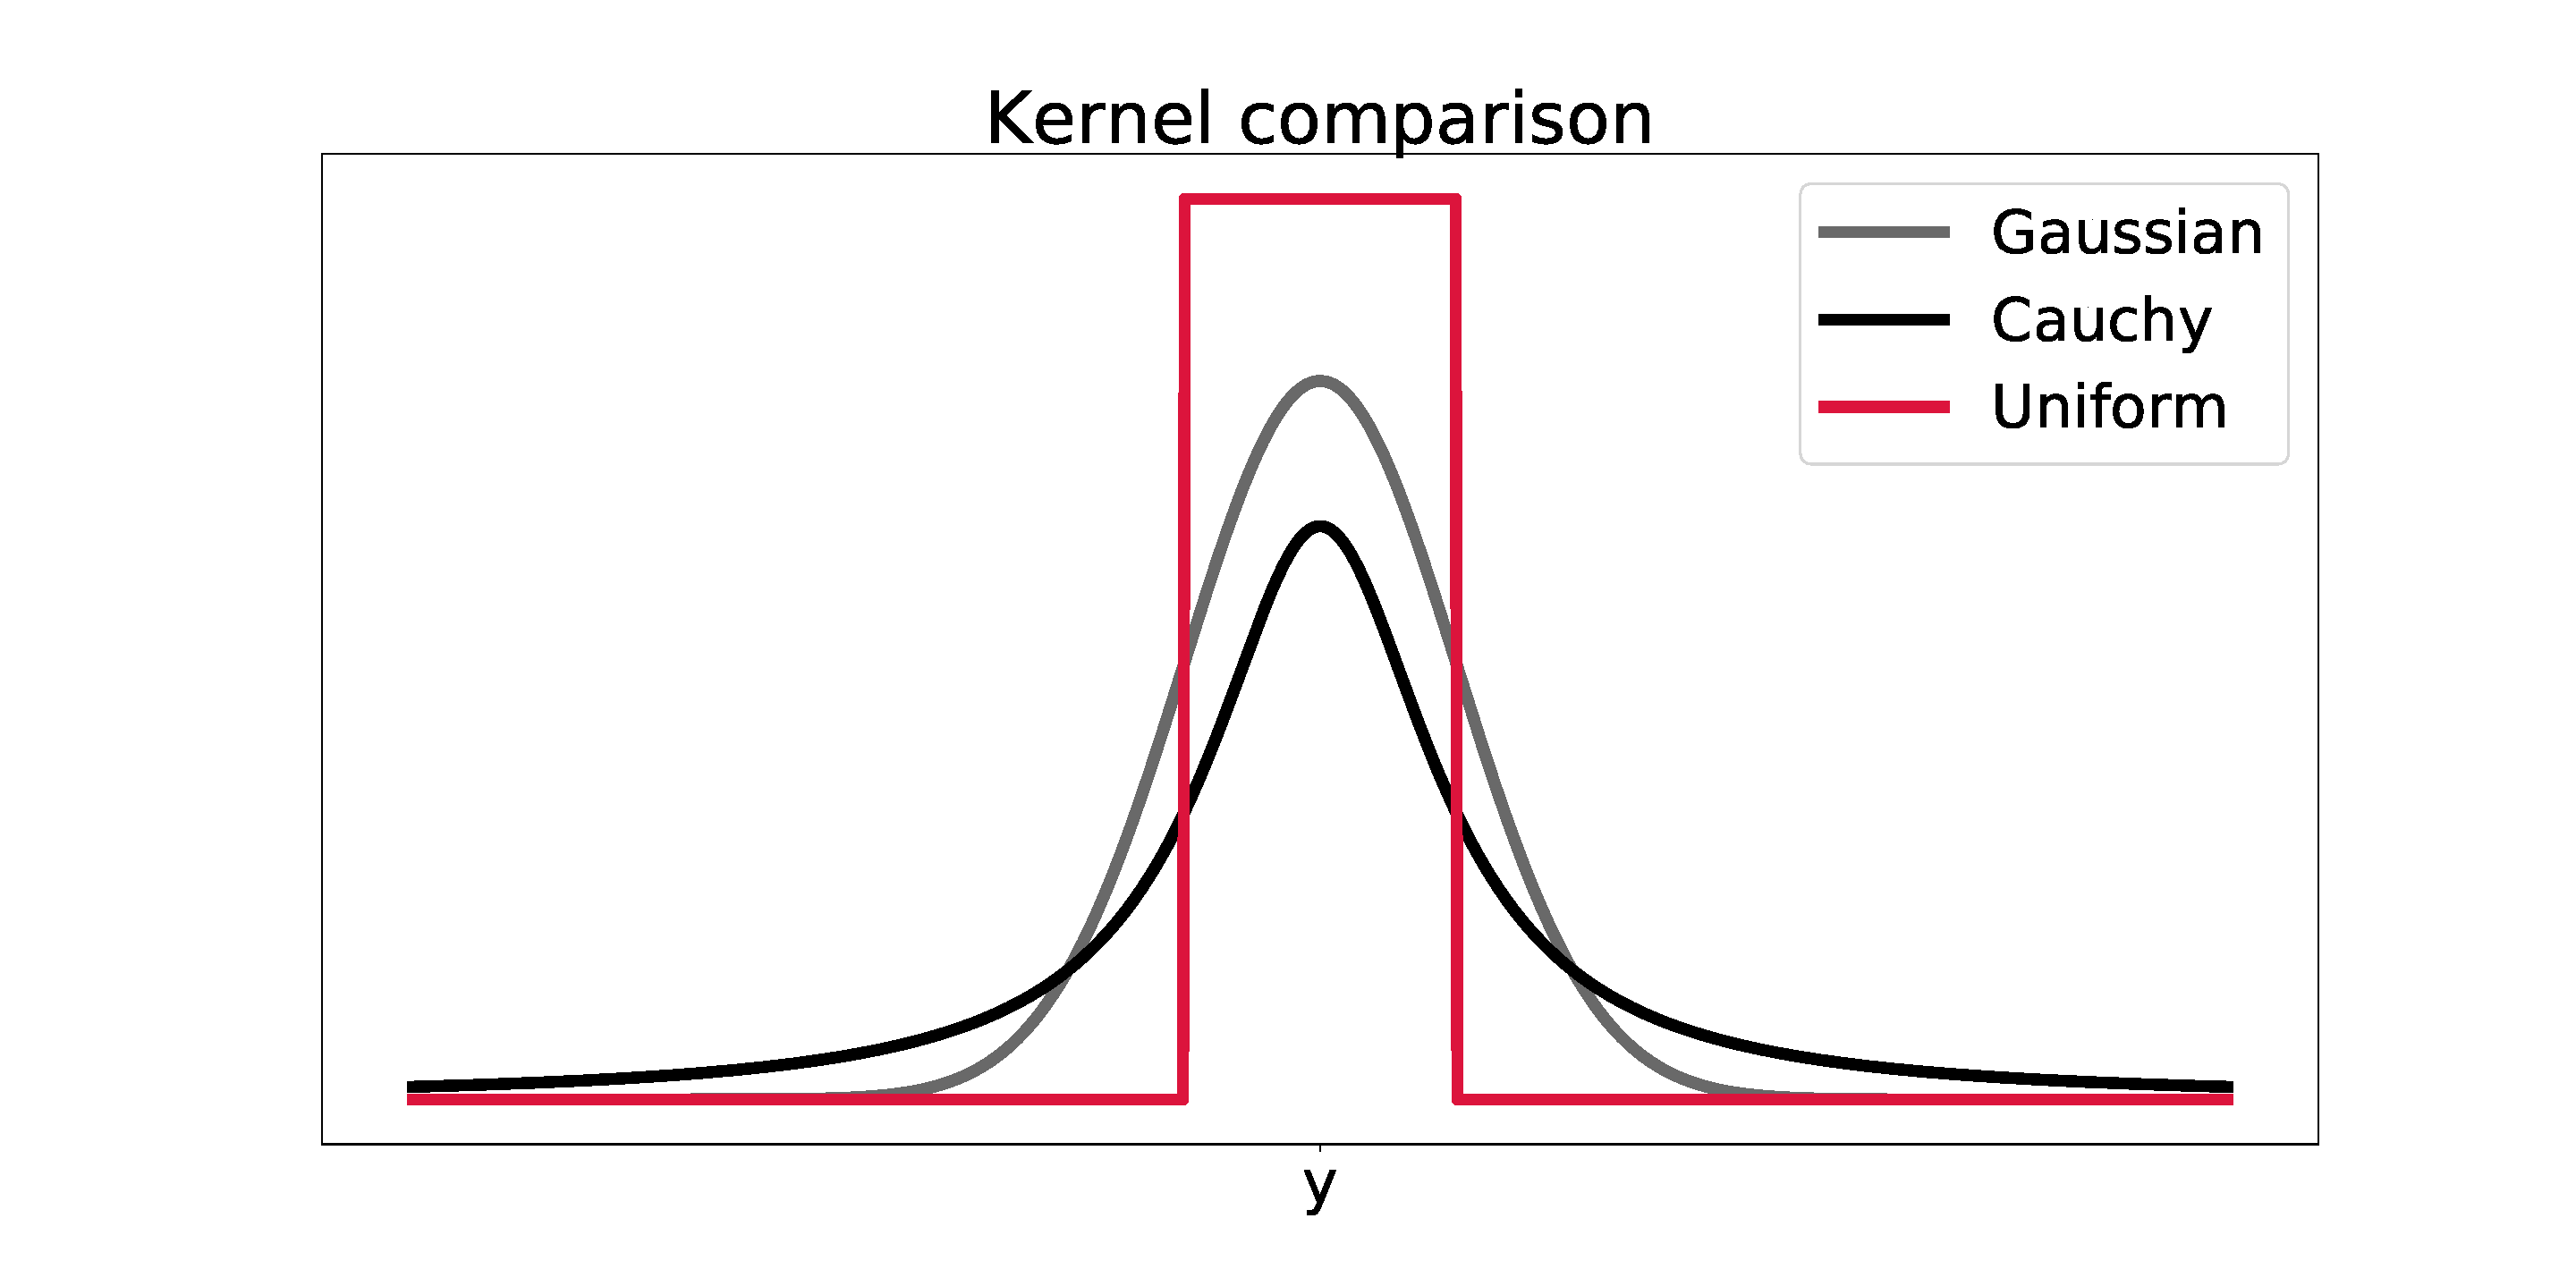
\includegraphics[width=\linewidth]{kernels}
    \caption{The Gaussian, Cauchy and uniform kernel functions centered at $y = 0$ with width $\epsilon = 3$.}
    \label{fig:kernels}
\end{figure}


The Noisy ABC procedure described above is then naturally generalized by perturbing the observations by samples from a given kernel, instead of the uniform distribution in a ball.


\paragraph{Kernel width tuning}
In this paragraph, we address the issue of tuning the kernel width $\epsilon$. Since the previous section has shown that the indicator function $\I_{\A_{\epsilon, \by}}$ is recovered by a particular kernel, the method also applies to the standard ABC formulation.

A careful setting of $\epsilon$ is necessary. When the kernel width is too low, most of the $N$ generated pseudo-observations are assigned with low probabilities, and the importance weights are close to zero. On the other hand, when the width is too high, even outlying pseudo-observations are assigned a non-trivial probability and shift the filter to incorrect values. In addition, the kernel becomes flat and close to the uniform variant. A manual setting of $\epsilon$ is thus a non-obvious task without any guidelines in the data. Additionally, the width should somehow reflect the filter evolution over time, since all observations $\by_t$ are different and may require different kernel widths.

In this thesis, we adopt a procedure described by \cite{dedecius}, which is briefly reviewed below. More details can be found in the original paper.

The method is based on the idea that the true observation model $\obs_t(\by_t \mid \bx_t, \btheta)$ should cover a given number of generated pseudo-observations $\bu_t^{(i)}, i = 1, \ldots, N$ by a $100p\%$ high probability region ($p$-HPR), where $p \in \left(0, 1\right)$ is a given constant. If this is true, the pseudo-observations can be expected to describe the distribution $\obs_t(\by_t \mid \bx_t, \btheta)$ sufficiently-well. As this distribution is not known, it is approximated by the kernel $\kappa$ evaluated at $\bu_t^{(i)}, i = 1, \ldots, N$.

As given in \eqref{eq:abc-likelihood-kernel}, the kernel is evaluated at each pseudo-observation $\bu_t^{(i)}, i = 1, \ldots, N$ while centered at $\by_t$. We then need to tune the width at time $t$, denoted $\epsilon_t$, so that a given fraction $\frac{\alpha}{N}$ of the pseudo-observations is covered by the $p$-HPR of the kernel. For the procedure to work, the kernel function $\kappa$ must be invariant under translation and scaling, i.e., belong to the location-scale family of distributions. Many popular kernels including the three discussed above, belong to this family.

The tuning procedure involves two steps:
\begin{enumerate}
    \item Identify $u_t^{[\alpha]}$, the $\alpha$th closest pseudo-observation to $y_t$.
    \item Center the kernel $\kappa$ at $y_t$ and set the width $\epsilon_t$ so that
    \begin{equation} \label{eq:kernel-tuning-integral}
    \left| \int_{y_t}^{u_t^{[\alpha]}} \kappa(u_t; y_t, \epsilon_t) \; \dx{u_t} \right| = \frac{p}{2},
    \end{equation}
    meaning that $u_t^{[\alpha]}$ lies at the boundary of the $p$-HPR of $\kappa(\cdot; y_t, \epsilon_t)$.
\end{enumerate}
These two steps are visualized in \autoref{fig:kernel-tuning}. In the case of multidimensional $\by_t$ and $\bu_t$, this procedure is performed coordinate-wise. 

\begin{figure}[ht]
    \centering
    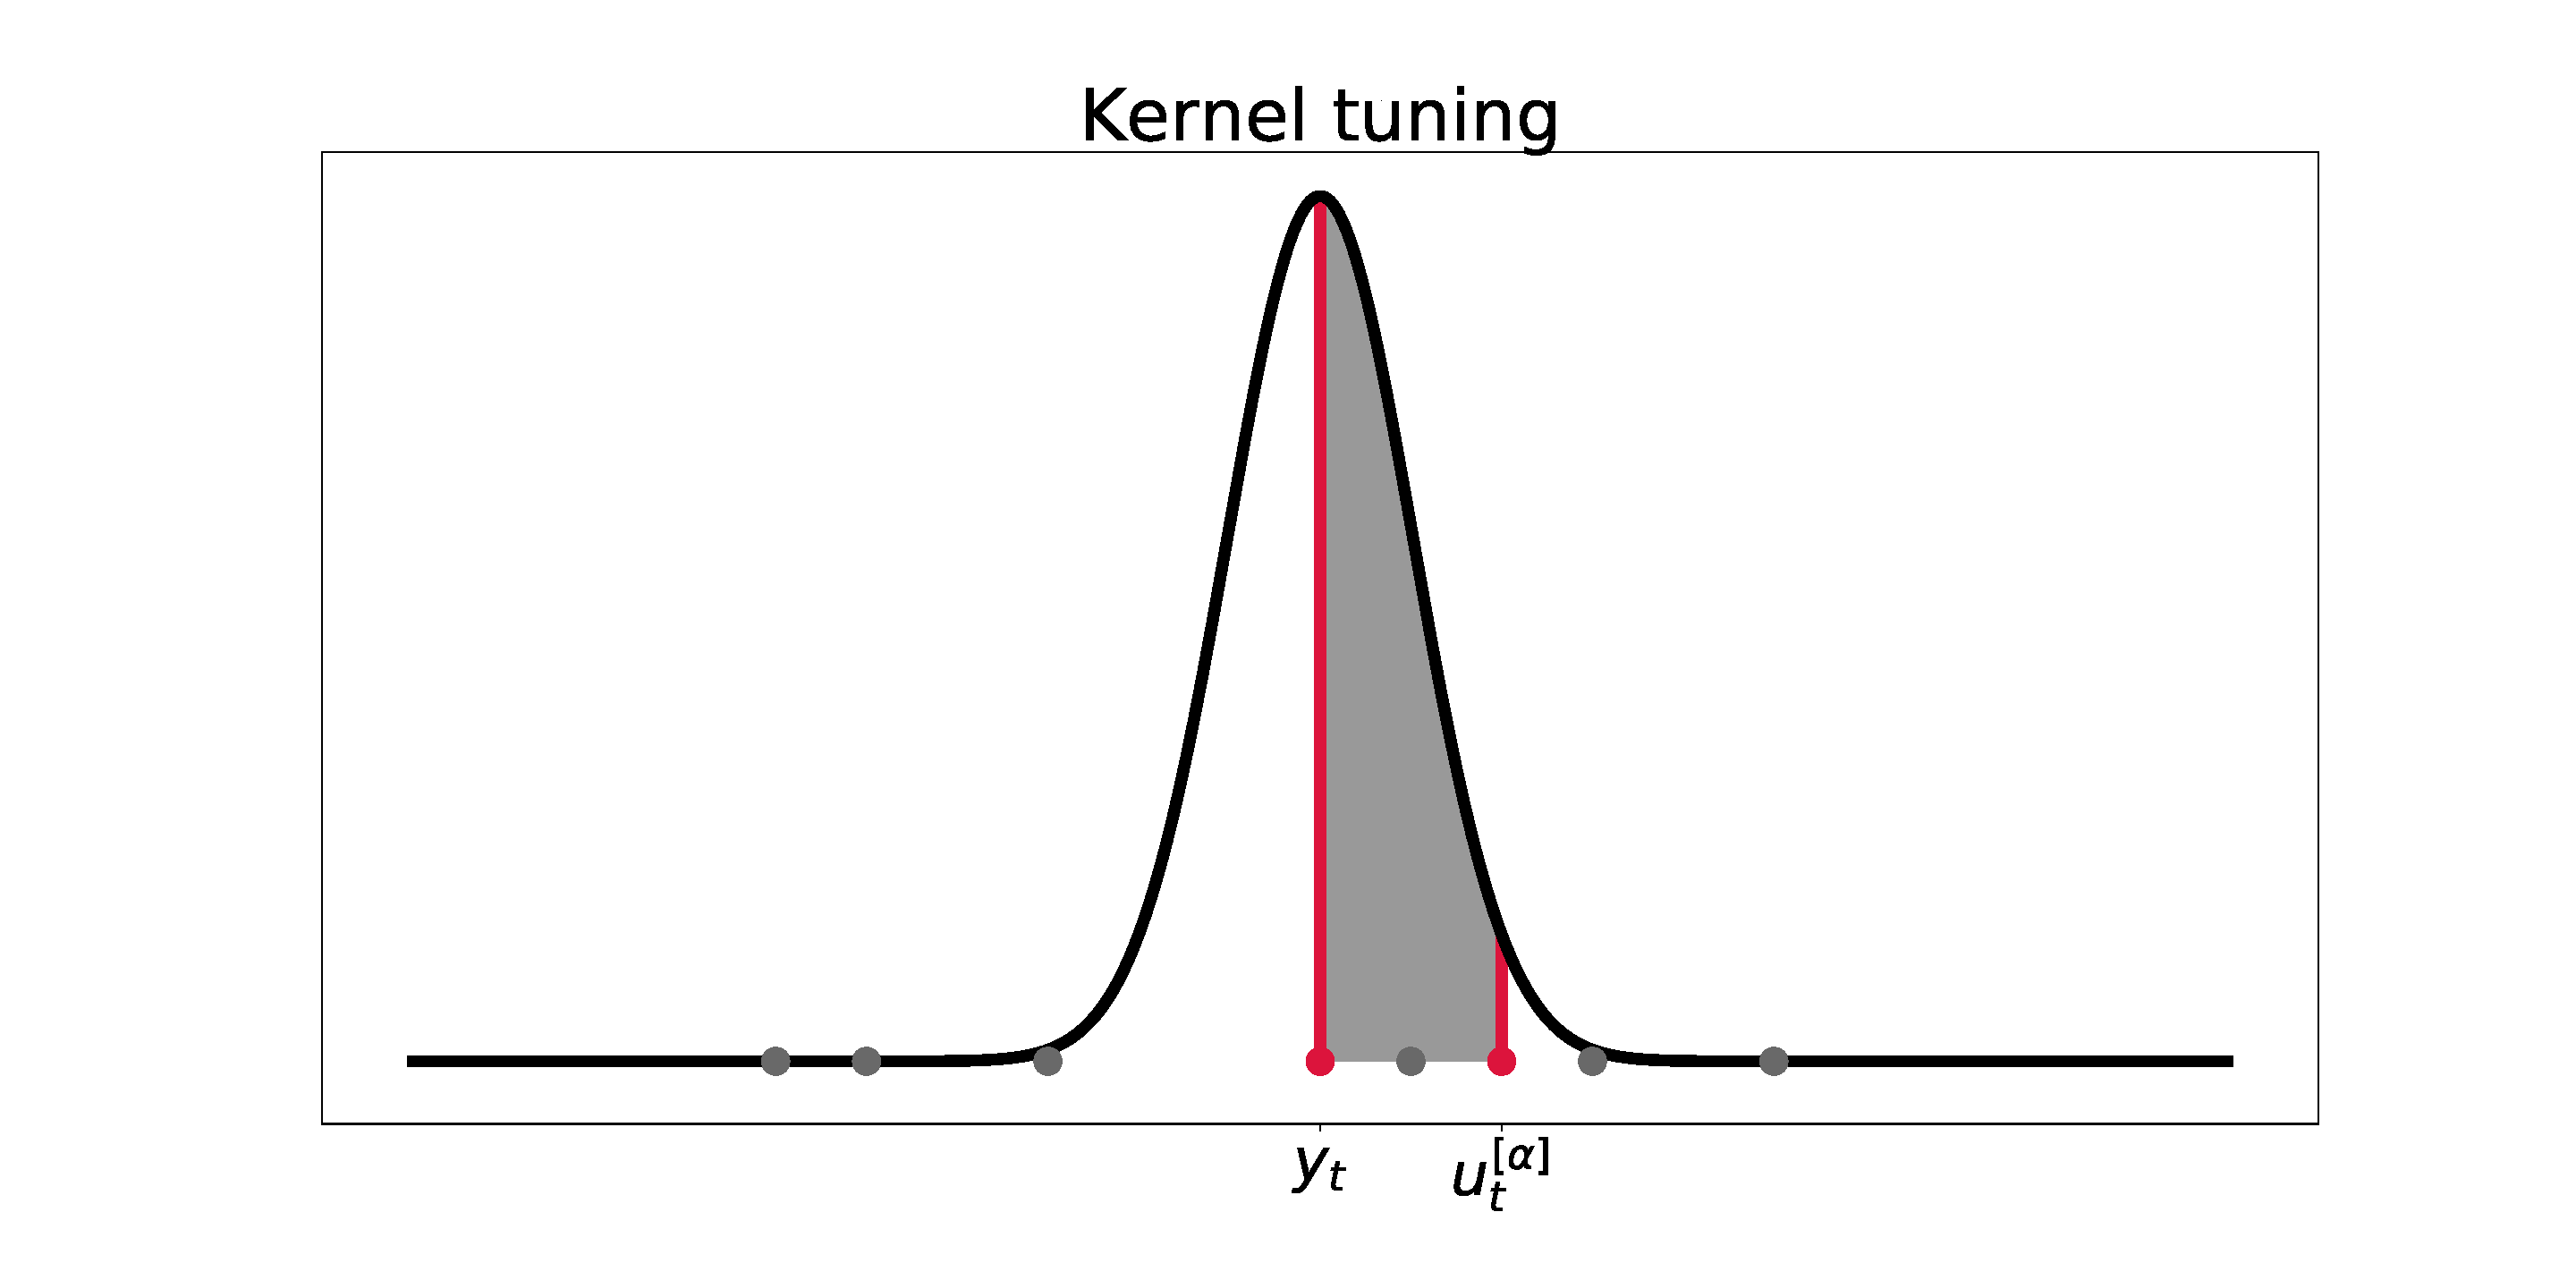
\includegraphics[width=\linewidth]{kernel_tuning}
    \caption{Visualization of the kernel tuning procedure. In this picture, ${\alpha = 2}$, ${p = 0.95}$, and the kernel is Gaussian. Plotted is the kernel along with a number of pseudo-observations $u_t^{(i)}$ and the true measurement $y_t$. Equation \eqref{eq:kernel-tuning-integral} states that the shaded area has volume $p/2 = 0.475$.}
    \label{fig:kernel-tuning}
\end{figure}

The meaning of equation \eqref{eq:kernel-tuning-integral} is that $u_t^{[\alpha]}$ is either the $\frac{1-p}{2}$-quantile or the $\frac{1+p}{2}$-quantile of $\kappa(\cdot; y_t, \epsilon_t)$, depending on whether $u_t^{[\alpha]} \leq y_t$ or $u_t^{[\alpha]} \geq y_t$. If we restrict ourselves to symmetric kernels, we may get rid of this case division by exploiting kernel symmetry.

Let $F$ denote the cumulative distribution function of the kernel $\kappa(\cdot; 0, 1)$ centered at 0 with width $\epsilon = 1$. Let its quantile function be denoted by $F^{-1}$. From $\kappa$ belonging to the location-scale family, we get that the quantile function of a general kernel $\kappa(\cdot; y_t, \epsilon_t)$ is
\begin{equation} \label{eq:location-scale-quantile}
Q(\beta) = y_t + \epsilon_t F^{-1}(\beta), \quad \beta \in \left(0, 1\right).
\end{equation}
As \eqref{eq:kernel-tuning-integral} and the assumed kernel symmetry require $\left| u_t^{[\alpha]} \right|$ to be the $\frac{1+p}{2}$-quantile of $\kappa(\cdot; y_t, \epsilon_t)$, we can substitute $u_t^{[\alpha]}$ for $Q(\beta)$ in \eqref{eq:location-scale-quantile} and solve for $\epsilon_t$, obtaining
\begin{equation} \label{eq:kernel-tuning}
\epsilon_t = \frac{\left| u_t^{[\alpha]} - y_t \right|}{F^{-1}(\frac{1+p}{2})},
\end{equation}
where the absolute value comes from the kernel being symmetric, so it is irrelevant whether we consider pseudo-observations lower or greater than the true observation $y_t$. The quantile function $F^{-1}$ is uniquely associated with each kernel, and the only free parameters are $\alpha$ and $p$.


\section{Likelihood estimate through ABC} \label{sec:abcmh}
The main contribution of this thesis is the utilization of the ABC framework to make inference possible even in SSMs with an unknown observation model. We have already derived all the necessary elements needed to state our main result. It remains to put them together by formalizing the entire inference process using ABC as a likelihood estimator.

\autoref{alg:abc-filter-complete} presents a modification of the particle filter which uses the ABC approximation as a surrogate for the unknown observation model. Compared to the particle filter, our formulation is applicable even when the observation model $\obs_t(\by_t \mid \bx_t, \btheta)$ is not given as a probability density. Unlike the basic ABC filter described in \autoref{alg:abc-filter}, our variant employs kernel functions to measure observation similarity, reflecting the fact that the closer a pseudo-measurement is to the true observation, the higher weight it should be assigned. In addition, we account for automatic tuning of the kernel widths by adapting them so that they cover a sufficient number of the simulated pseudo-measurements.

\begin{algorithm}[ht]
    \caption{ABC-based filter with automatic kernel tuning}
    \label{alg:abc-filter-complete}
    \begin{algorithmic}[1]
        \Input $\text{Number of particles } N,\ \text{current parameter value } \btheta, \text{ HPR } p, \newline \text{number of covered pseudo-observations } \alpha,\ \left\{\by_1, \ldots, \by_T\right\}.$
        
        \State $\text{Sample } \bx_0^{(i)} \sim \sprior(\cdot \mid \btheta), \quad i = 1, \ldots, N.$ \Comment{Initialize $N$ particles.}
        
        \State $w_0^{(i)} \gets \frac{1}{N}, \quad i = 1, \ldots, N.$ \Comment{Initialize uniform weights.}
        
        \For{$t = 1\ \mathbf{to}\ T$}
        \State $\text{Sample } \bx_t^{(i)} \sim \trans_t(\bx_t \mid \bx_{t-1}^{(i)}, \btheta), \quad i = 1, \ldots, N.$ \Comment{Sample $N$ new particles.}
        
        \State $\text{Simulate } \bu_t^{(i)} \text{ from } \obs_t(\cdot \mid \bx_t^{(i)}), \quad i = 1, \ldots, N.$ \Comment{Simulate $N$ pseudo-observations.}
        
        \State $\text{Identify } \bu_t^{[\alpha]}.$ \Comment{Find the $\alpha$th closest pseudo-observation to $\by_t$.}
        
        \State $\epsilon_t \gets \frac{\left| u_t^{[\alpha]} - y_t \right|}{F^{-1}(\frac{1+p}{2})}$ \Comment{Set the kernel width at time $t$ according to \eqref{eq:kernel-tuning}.}
        
        \State $\text{Set } w_t^{(i)} \propto \kappa(\bu_t^{(i)}; \by_t, \epsilon_t) w_{t-1}^{(i)}, \quad i = 1, \ldots, N.$
        
        \State $\text{Resample } \bx_t^{(i)} \text{ and reset } w_t^{(i)} \text{ using \autoref{alg:resampling}}, \quad i = 1, \ldots, N.$
        \EndFor
    \end{algorithmic}
\end{algorithm}

Finally, \autoref{alg:marginal-metropolis-hastings-abc} reformulates the marginal Metropolis-Hastings according to the ABC methodology. Under the new formulation, the estimator $\widehat{\aux}$ of $p(\by_{1:T} \mid \btheta)$ is constructed by evaluating \eqref{eq:abc-likelihood-kernel} on a set of importance weights calculated by \autoref{alg:abc-filter-complete}. The result is used to compute the acceptance probability which again controls whether a proposed $\btheta^\prime$ and the corresponding $\widehat{\aux}^\prime$ are accepted or not.

\begin{algorithm}[ht]
    \caption{Marginal Metropolis-Hastings with ABC filter}
    \label{alg:marginal-metropolis-hastings-abc}
    \begin{algorithmic}[1]
        \Input $\text{Number of samples } M,\ \left\{\by_1, \ldots, \by_T\right\}.$
        
        \State $\text{Initialize } \btheta^{(0)}.$
        \State $\text{Run \autoref{alg:abc-filter-complete} with } \btheta^{(0)} \text{ to obtain the weights } w_{0,t}^{(i)}, \quad t = 1, \ldots, T,\ i = 1, \ldots, N.$
        \State $\text{Calculate } \widehat{\aux}^{(0)} \text{ according to \eqref{eq:abc-likelihood-kernel} using } w_{0,t}^{(i)}.$
        
        \For{$m = 1\ \mathbf{to}\ M$}
        \State $\text{Sample } \btheta^\prime \sim \prop(\cdot \mid \btheta^{(m-1)}).$
        \State $\text{Run \autoref{alg:abc-filter-complete} with } \btheta^\prime \text{ to obtain the weights } w_{m,t}^{(i)}, \quad t = 1, \ldots, T, \ i = 1, \ldots, N.$
        \State $\text{Calculate } \widehat{\aux}^\prime \text{ according to \eqref{eq:abc-likelihood-kernel} using } w_{m,t}^{(i)}.$
        \State $\text{Calculate the aceptance probability } $ \begin{equation*} \label{eq:acceptance-probability-tractable-abc}
        \alpha = \min \left\{1, \frac{\widehat{\aux}^\prime \pprior(\btheta^\prime)}{\widehat{\aux}^{(m-1)} \pprior(\btheta^{(m-1)})} \frac{\prop(\btheta^{(m-1)} \mid \btheta^\prime)}{\prop(\btheta^\prime \mid \btheta^{(m-1)})} \right\}.
        \end{equation*}
        \State $\text{Sample } u \sim \mathcal{U}(0,1).$
        \If {$u \leq \alpha$}
        \State $\left( \btheta^{(m)}, \widehat{\aux}^{(m)} \right) \gets \left( \btheta^\prime, \widehat{\aux}^\prime \right)$ \Comment{With probability $\alpha$, accept the proposed sample.}
        \Else
        \State $\left( \btheta^{(m)}, \widehat{\aux}^{(m)} \right) \gets \left( \btheta^{(m-1)}, \widehat{\aux}^{(m-1)} \right)$ \Comment{With probability $1 - \alpha$, reject the proposed sample.}
        \EndIf
        \EndFor
        
        \Output $\left\{ \btheta^{(1)}, \ldots, \btheta^{(M)} \right\}$
    \end{algorithmic}
\end{algorithm}
\chapter{Applications}
\label{chap:applications}

In this chapter, we apply the models developed earlier to two selected problems. The first problem is the Lotka-Volterra model described in \autoref{sec:lotka-volterra}, the second is a simple model for auto-regulation in prokaryotes considered in \autoref{sec:autoregulation}. The particle filter-based approach is compared with the one depending on ABC methods in various settings and model misspecifications.

Both problems require simulating reactions in order to propagate the system states through time. This is done with the help of the Gillespie algorithm, which is first described in \autoref{sec:gillespie}.

\section{Preliminary: the Gillespie algorithm} \label{sec:gillespie}
The Gillespie algorithm \citep{gillespie1, gillespie2} is used to simulate a stochastic process describing the time evolution of a system of reactions. The discussion given here follows \cite{wilkinson-book}.

\paragraph{Time evolution of a reaction system}
Consider a system consisting of $u$ species $\mathcal{X}_1, \ldots, \mathcal{X}_u$ and $v$ reactions $\mathcal{R}_1, \ldots, \mathcal{R}_v$. The species can describe literal animal species, as is the case in the Lotka-Volterra model in \autoref{sec:lotka-volterra}, or individual molecule types, as in \autoref{sec:autoregulation}. The reactions describe the interactions between these species through time.

Let the number of molecules (or individuals, in case of animal species) of the species $\mathcal{X}_i$ at time $t$ be denoted by $X_{i,t}$, and let $\bm{X}_t = \left(X_{1,t}, \ldots, X_{u,t}\right)^\intercal$. Additionally, let the number of reactions of type $\mathcal{R}_i$ which occurred in a time window $(0, t]$ be denoted by $R_{i,t}$, and let $\bm{R}_t = \left(R_{1,t}, \ldots,R_{v,t}\right)^\intercal$. The evolution of the system from time 0 to time $t$ is described by the equation
\begin{equation} \label{eq:system-evolution}
\bm{X}_t - \bm{X}_0 = \mathbb{S}\bm{R}_t,
\end{equation}
where $\mathbb{S} \in \R^{u \times v}$ is called the stoichiometry matrix of the system, and describes the difference in the number of molecules of each species after each reaction occurs. To gain insight into the meaning of $\mathbb{S}$, it is instructive to write it as
\begin{equation*}
\mathbb{S} = \mathbb{P}_\text{post} - \mathbb{P}_\text{pre},
\end{equation*}
where the element $(i,j)$ of $\mathbb{P}_\text{pre}$ denotes the number of molecules of $\mathcal{X}_i$ before a reaction of type $\mathcal{R}_j$ takes place, and the element $(i,j)$ of $\mathbb{P}_\text{post}$ describes the same quantity \emph{after} it takes place. Equation \eqref{eq:system-evolution} can then be written as
\begin{equation*}
\bm{X}_t = \bm{X}_0 + \left(\mathbb{P}_\text{post} - \mathbb{P}_\text{pre}\right) \bm{R}_t,
\end{equation*}
and describes the net gain in the number of molecules of each species, given their initial numbers, and accounting for their increase/decrease when a number of reactions of each type occurs.

In addition, each reaction $\mathcal{R}_i$ has a stochastic rate constant $c_i$ and a rate law (also called the hazard function) $h_i(\bm{X}_t, c_i)$ associated with it. The interpretation of the hazard function is such that $h_i(\bm{X}_t, c_i) \dx{t}$ is the probability of a reaction of type $\mathcal{R}_i$ occurring in a time interval $(t, t + \dx{t}]$, conditionally on the system being in state $\bm{X}_t$. Such a situation is described by an exponential distribution -- the time to the event of a reaction of type $\mathcal{R}_i$ occurring, assuming no other reaction is taking place, is distributed according to ${\mathcal{E}\mathit{xp}\left(h_i(\bm{X}_t, c_i)\right)}$. This is however a convenient simplification, since multiple reactions are typically occurring at the same time.

\paragraph{The Gillespie algorithm}
In a system with $v$ reactions and their hazard functions $h_i(\bm{X}_t, c_i)$, the hazard of \emph{some} reaction occurring is
\begin{equation*}
h_0(\bm{X}_t, \bm{c}) = \sum_{i=0}^v h_i(\bm{X}_t, c_i),
\end{equation*}
where $\bm{c} = \left(c_1, \ldots, c_v\right)^\intercal$. The time to the next reaction is then distributed according to $\mathcal{E}\mathit{xp}\left(h_0(\bm{X}_t, \bm{c})\right)$. The particular reaction type is a random variable with a categorical distribution $\mathcal{C}\mathit{at}\left(\widetilde{h}_1(\bm{X}_t,c_1), \ldots, \widetilde{h}_v(\bm{X}_t,c_v)\right)$, where $\displaystyle \widetilde{h}_i(\bm{X}_t,c_i) = \frac{h_i(\bm{X}_t,c_i)}{h_0(\bm{X}_t, \bm{c})}$.

With the above in mind, the Gillespie algorithm can now be formulated, and is given in \autoref{alg:gillespie}. Its purpose is to simulate the state evolution \eqref{eq:system-evolution} for a given time horizon $T$ while accounting for the randomness in the time until a reaction of a particular type takes place. For the purpose of this algorithm, denote the columns of the stoichiometry matrix $\mathbb{S}$ by $\bm{S}^i, \quad i = 1, \ldots, v$.
\begin{algorithm}[ht]
    \caption{Gillespie algorithm}
    \label{alg:gillespie}
    \begin{algorithmic}[1]
        \Input $\text{Time horizon } T, \text{ rate constants } \bm{c} = \left(c_1, \ldots, c_v\right)^\intercal,\ \text{initial molecule numbers } \bm{X}_0.$
        
        \State $t \gets 0$
        
        \State $\bm{X}_t \gets \bm{X}_0$
        
        \While{$t \leq T$}
            \State $\text{Calculate } h_i(\bm{X}_t, c_i), \quad i = 1, \ldots, v.$
            \State $h_0(\bm{X}_t, \bm{c}) \gets \sum_{i=1}^v h_i(\bm{X}_t, c_i)$
            \State $\text{Calculate } \displaystyle \widetilde{h}_i(\bm{X}_t,c_i) = \frac{h_i(\bm{X}_t,c_i)}{h_0(\bm{X}_t, \bm{c})}, \quad i = 1, \ldots, v.$
            \State $\text{Sample } \dx{t} \sim \mathcal{E}\mathit{xp}\left(h_0(\bm{X}_t, \bm{c})\right).$ \Comment{Simulate the time to the next reaction.}
            \State $\text{Sample } i \sim \mathcal{C}\mathit{at}\left(\widetilde{h}_1(\bm{X}_t,c_1), \ldots, \widetilde{h}_v(\bm{X}_t,c_v)\right).$ \Comment{Simulate the reaction type.}
            \State $\bm{X}_{t + \dx{t}} \gets \bm{X}_t + \bm{S}^i$ \Comment{Update the state according to the reaction $i$.}
            \State $t \gets t + \dx{t}$
        \EndWhile
        
        \Output $\text{Final state } \bm{X}_t, \text { final time } t.$
    \end{algorithmic}
\end{algorithm}

The algorithm is usually the bottleneck of most simulations, and must be implemented carefully; otherwise, the simulation becomes unacceptably slow. The final time $t$ is at the output as well, since it may exceed the horizon $T$. If the algorithm is run consecutively during a simulation, the interest is to follow the previous run by starting at its final time $t$.

\section{Lotka-Volterra model} \label{sec:lotka-volterra}
\paragraph{Problem description}
The first considered problem is the Lotka-Volterra model \citep{lotka, volterra}. The system describes a simplified time interaction of a population consisting of a predator and prey species. Denoting the prey species by $\mathcal{X}_1$ and the predator species by $\mathcal{X}_2$, the system can be described by the reactions
\begin{align}
\mathcal{R}_1:\quad & \mathcal{X}_1 \to 2 \mathcal{X}_1, \label{eq:lv1} \\
\mathcal{R}_2:\quad & \mathcal{X}_1 + \mathcal{X}_2 \to 2 \mathcal{X}_2, \label{eq:lv2} \\
\mathcal{R}_3:\quad & \mathcal{X}_2 \to \emptyset. \label{eq:lv3}
\end{align}
Equation \eqref{eq:lv1} describes the reproduction of the prey species. Equation \eqref{eq:lv2} describes the interaction between the predator and the prey where a predator consumes an individual of the prey species and produces an offspring. Equation \eqref{eq:lv3} describes the extinction of the predator species when no prey is present.

The state of the system at time $t$ is $\bm{X}_t = \left(X_{1,t}, X_{2,t}\right)^\intercal$. The stoichiometry matrix is given by
\begin{equation*}
\mathbb{S} = \begin{pmatrix}
1 & -1 & 0 \\
0 & 1 & -1 \\
\end{pmatrix},
\end{equation*}
and the hazard functions vector is $\bm{h}(\bm{X}_t, \bm{c}) = \left(c_1 X_{1,t}, c_2 X_{1,t} X_{2,t}, c_3 X_{2,t}\right)^\intercal$ \citep{wilkinson}. Although simple to describe, this model is analytically intractable \citep{wilkinson-book}.

For the inference problem, we consider the unknown parameters to be $\btheta = \left(c_1, c_2, c_3\right)^\intercal$, and the state at time $t$ to be $\bx_t = \left(X_{1,t}, X_{2,t}\right)$. Since the rate constants $c_1, c_2, c_3$ are by definition positive, we are working in the log space to avoid restricting ourselves to positive support distributions. The model is specified by the following:
\begin{equation*}
\begin{split}
\sprior(x_{1,0} \mid \btheta) &= \mathcal{P}\mathit{o}\left(50\right), \\
\sprior(x_{2,0} \mid \btheta) &= \mathcal{P}\mathit{o}\left(100\right), \\
\trans_t(\bx_t \mid \bx_{t-1}, \btheta) & \text{ is simulated using \autoref{alg:gillespie} }, \\
\obs_t(\by_t \mid \bx_{t}, \btheta) &= \mathcal{N}_2\left(\bx_t, 10^2\right).
\end{split}
\end{equation*}
The parameter prior and the Metropolis-Hastings proposal are additionally given by
\begin{equation*}
\begin{split}
\pprior(\log c_i) &= \mathcal{U}\left(-7, 2\right), \quad i = 1, 2, 3, \\
\prop(\btheta^\prime \mid \btheta) &= \mathcal{N}_3\left(\btheta, \text{diag}\left(0.01, 0.01, 0.01\right)\right).
\end{split}
\end{equation*}
The initial parameters are $\btheta^{(0)} = \left(1, 0.005, 0.6\right)^\intercal$. We are working with a dataset simulated using \autoref{alg:gillespie} ran so that it outputs 16 observations $\by_t$, starting from the same parameters $\btheta^{(0)}$. The inference is started in the correct parameters and applied on a short sequence only; its purpose is only to demonstrate that the algorithm is able to identify these parameters.

We apply the marginal Metropolis-Hastings algorithm depending on the particle filter as well as the one utilizing ABC methods. Both algorithms are ran for $M = 50000$ samples with $N = 100$ particles. Additionally, the number of covered pseudo-observations in the ABC formulation is $\alpha = 95$ and the volume of the p-HPR is $p = 0.95$.

\paragraph{Correctly specified observation model}

\paragraph{Misspecified observation model}

\section{Prokaryotic auto-regulation model} \label{sec:autoregulation}
\paragraph{Problem description}

\paragraph{Correctly specified observation model}

\paragraph{Misspecified observation model}
\chapter{Conclusion and future work}
\label{chap:conclusion}

In this thesis, we considered the problem of static parameter inference in state-space models. We approached the problem from a Bayesian viewpoint, formulating a prior density and inferring a posterior distribution. The inference process is complicated by the likelihood of the state-space model being intractable, which prevents the application of standard Markov Chain Monte Carlo (MCMC) methods.

To address this issue, we initially considered the particle filter. First, we derived the filter through importance sampling, and listed some of its properties. We then described how we can estimate the model likelihood through the particle filter without affecting the asymptotic properties of the MCMC sampler.

The complication is that the particle filter requires the observation model to be completely determined. In applications, we often do not possess knowledge about the exact probabilistic form of this observation density. Instead, we have a means to generate observations from the latent states, typically by a (differential) equation or a simulation. In this case, we may apply Approximate Bayesian Computation techniques to instead approximate the likelihood through simulations.

We derived the exact form of this filter, as well as the use of kernel functions to measure similarity between true and simulated observations. We adopted a technique to tune the kernel widths so that they cover a sufficient number of simulated measurements.

The particle filter and ABC-based methods were compared on two examples, both requiring the simulation of stochastic reactions using the Gillespie algorithm. The first experiment was the Lotka-Volterra model, the second one a simplified model for prokaryotic auto-regulation. We compared the two approaches in well-specified as well as in misspecified observation model scenarios.

In both cases, the particle filter worked well under the correct model, and completely collapsed under model misspecification. The ABC-based method does not suffer from this collapse, but as an approximation, performs necessarily worse than the particle filter. This is clear especially in the auto-regulation model, which poses a considerably more difficult task than the Lotka-Volterra system.

In future, the possibility to use multidimensional kernel functions could be considered. The kernel width tuning procedure utilized in this thesis has been derived in context of one-dimensional kernels, and applied coordinate-wise in case of multidimensional observations. As a consequence, the individual observation vector elements are assumed independent. By allowing to model them in a multidimensional settings, one could also exploit their dependencies.

If applications to more complicated biological systems was of interest, one should study more sophisticated ways of simulating the latent states. The Gillespie algorithm is still a naïve method, and fails to cover the details present in systems as complex as those found in molecular biology.


% Bibliography
\bibliographystyle{abbrvnat}
\bibliography{tex/references}


% Appendices
%\appendix
%\chapter{Real events used for evaluation}
%\label{app:real-events}
%\input{tex/chapters/appendix_real_events}

%\chapter{DVD contents}
%\input{tex/chapters/dvd_contents}


\end{document}